\input{setup/preamble.tex}% package inclusion and set up of the document

%Creates the aau titlepage
\newcommand{\aautitlepage}[3]{%
  {
    %set up various length
    \ifx\titlepageleftcolumnwidth\undefined
      \newlength{\titlepageleftcolumnwidth}
      \newlength{\titlepagerightcolumnwidth}
    \fi
    \setlength{\titlepageleftcolumnwidth}{0.5\textwidth-\tabcolsep}
    \setlength{\titlepagerightcolumnwidth}{\textwidth-2\tabcolsep-\titlepageleftcolumnwidth}
    %create title page
    \thispagestyle{empty}
    \noindent%
    \begin{tabular}{@{}ll@{}}
      \parbox{\titlepageleftcolumnwidth}{
        \iflanguage{danish}{%
          \includegraphics[width=\titlepageleftcolumnwidth]{setup/aau_logo_da.pdf}
        }{%
          \includegraphics[width=\titlepageleftcolumnwidth]{setup/aau_logo_en.pdf}
        }
      } &
      \parbox{\titlepagerightcolumnwidth}{\raggedleft\sf\small
        #2
      }\bigskip\\
       #1 &
      \parbox[t]{\titlepagerightcolumnwidth}{%
      \textbf{Abstract:}\smallskip\par
        \fbox{\parbox{\titlepagerightcolumnwidth-2\fboxsep-2\fboxrule}{%
          #3
        }}
      }\\
    \end{tabular}
    \vfill
    \vspace{-0.5cm}
    \iflanguage{danish}{%
      \noindent{\footnotesize\emph{Rapportens indhold er frit tilgængeligt, men offentliggørelse (med kildeangivelse) må kun ske efter aftale med forfatterne.}}
    }{%
      \noindent{\footnotesize\emph{The content of this report is freely available, but publication (with reference) may only be pursued due to agreement with the author.}}
    }
    \clearpage
  }
}

%Create english project info
\newcommand{\englishprojectinfo}[8]{%
  \parbox[t]{\titlepageleftcolumnwidth}{
    \textbf{Title:}\\ #1\bigskip\par
    \textbf{Theme:}\\ #2\bigskip\par
    \textbf{Project Period:}\\ #3\bigskip\par
    \textbf{Project Group:}\\ #4\bigskip\par
    \textbf{Participant(s):}\\ #5\bigskip\par
    \textbf{Supervisor(s):}\\ #6\bigskip\par
    \textbf{Copies:} #7\bigskip\par
    \textbf{Page Numbers:} Fucking mange!\bigskip\par
    \textbf{Date of Completion:}\\ #8
  }
}

%Create danish project info
\newcommand{\danishprojectinfo}[8]{%
  \parbox[t]{\titlepageleftcolumnwidth}{
    \textbf{Title:}\\ #1\bigskip\par
    \textbf{Theme:}\\ #2\bigskip\par
    \textbf{Project Period:}\\ #3\bigskip\par
    \textbf{Project Group:}\\ #4\bigskip\par
    \textbf{Participants:}\\ #5\bigskip\par
    \textbf{Supervisor:}\\ #6\bigskip\par
    \textbf{Copies:} #7\bigskip\par
    \textbf{Page Numbers:} ??
    \bigskip\par
    \textbf{Date of Completion:}\\ #8
  }
}

%Nice-looking reference to other chapters
\newcommand{\chapref}[1]{Chapter \ref{#1}: \nameref{#1}}
\newcommand{\secref}[1]{Section \ref{#1}: \nameref{#1}}
\newcommand{\figref}[1]{\emph{Figure: \ref{#1}}}
\newcommand{\appref}[1]{\emph{Appendix \ref{#1}}}
\newcommand{\tabref}[1]{\emph{Table: \ref{#1}}}
\newcommand{\coderef}[1]{\emph{Listings: \ref{#1}}}
\renewcommand{\eqref}[1]{\emph{Equation: (\ref{#1})}}

\newcommand{\iic}[0]{I²C }

%%%%%%%%%%%%%%%%%%%%%%%%%%%%%%%%%%%%%%%%%%%%%%%%
% An example environment
%%%%%%%%%%%%%%%%%%%%%%%%%%%%%%%%%%%%%%%%%%%%%%%%
\theoremheaderfont{\normalfont\bfseries}
\theorembodyfont{\normalfont}
\theoremstyle{break}
\def\theoremframecommand{{\color{aaublue!50}\vrule width 5pt \hspace{5pt}}}
\newshadedtheorem{exa}{Example}[chapter]
\newenvironment{example}[1]{%
		\begin{exa}[#1]
}{%
		\end{exa}
}

\makeatletter
\newcommand{\ChapterOutsidePart}{%
   \def\toclevel@chapter{-1}\def\toclevel@section{0}\def\toclevel@subsection{1}}
\newcommand{\ChapterInsidePart}{%
   \def\toclevel@chapter{0}\def\toclevel@section{1}\def\toclevel@subsection{2}}
\makeatother

\usepackage{bookmark}

\usepackage{mathtools}
\DeclarePairedDelimiter{\ceil}{\lceil}{\rceil}








%Figure references:
%\newcommand{\figref}[1]{\textbf{figure \ref{#1}}}

%Figure references after full stop/period:
\newcommand{\Figref}[1]{\textbf{Figure \ref{#1}}}

%Table references:
\newcommand{\tableref}[1]{\textbf{table \ref{#1}}}

%Table references after full stop/period:
\newcommand{\Tableref}[1]{\textbf{Table \ref{#1}}}

%Units:
\newcommand{\unit}[1]{&& \left[\si{#1}\right]}

%Text:
\newcommand{\tx}[1]{\text{#1}}

%Equation references:
%1 equation:
\renewcommand{\eqref}[1]{\textbf{equation (\ref{#1})}}
%2 equations:
\newcommand{\eqrefTwo}[2]{\textbf{equation (\ref{#1})} and \textbf{(\ref{#2})}}
%3 equations:
\newcommand{\eqrefThree}[3]{\textbf{equation (\ref{#1})}, \textbf{(\ref{#2})} and \textbf{(\ref{#3})}}
%4 equations:
\newcommand{\eqrefFour}[4]{\textbf{equation (\ref{#1})}, \textbf{(\ref{#2})}, \textbf{(\ref{#3})} and \textbf{(\ref{#4})}}
%5 equations:
\newcommand{\eqrefFive}[5]{\textbf{equation (\ref{#1})}, \textbf{(\ref{#2})}, \textbf{(\ref{#3})}, \textbf{(\ref{#4})} and \textbf{(\ref{#5})}}
%6 equations:
\newcommand{\eqrefSix}[6]{\textbf{equation (\ref{#1})}, \textbf{(\ref{#2})}, \textbf{(\ref{#3})}, \textbf{(\ref{#4})}, \textbf{(\ref{#5})} and \textbf{(\ref{#6})}}
%7 equations:
\newcommand{\eqrefSeven}[7]{\textbf{equation (\ref{#1})}, \textbf{(\ref{#2})}, \textbf{(\ref{#3})}, \textbf{(\ref{#4})}, \textbf{(\ref{#5})}, \textbf{(\ref{#6})} and \textbf{(\ref{#7})}}

%Equation references after full stop/period:
%1 equation:
\newcommand{\Eqref}[1]{\textbf{Equation (\ref{#1})}}
%2 equations:
\newcommand{\EqrefTwo}[2]{\textbf{Equation (\ref{#1})} and \textbf{(\ref{#2})}}
%3 equations:
\newcommand{\EqrefThree}[3]{\textbf{Equation (\ref{#1})}, \textbf{(\ref{#2})} and \textbf{(\ref{#3})}}
%4 equations:
\newcommand{\EqrefFour}[4]{\textbf{Equation (\ref{#1})}, \textbf{(\ref{#2})}, \textbf{(\ref{#3})} and \textbf{(\ref{#4})}}
%5 equations:
\newcommand{\EqrefFive}[5]{\textbf{Equation (\ref{#1})}, \textbf{(\ref{#2})}, \textbf{(\ref{#3})}, \textbf{(\ref{#4})} and \textbf{(\ref{#5})}}
%5 equations:
\newcommand{\EqrefSix}[6]{\textbf{Equation (\ref{#1})}, \textbf{(\ref{#2})}, \textbf{(\ref{#3})}, \textbf{(\ref{#4})}, \textbf{(\ref{#5})} and \textbf{(\ref{#6})}}
%5 equations:
\newcommand{\EqrefSeven}[7]{\textbf{Equation (\ref{#1})}, \textbf{(\ref{#2})}, \textbf{(\ref{#3})}, \textbf{(\ref{#4})}, \textbf{(\ref{#5})}, \textbf{(\ref{#6})} and \textbf{(\ref{#7})}}% my new macros

\begin{document}
%%% Prereport %%%
\setlength\cftaftertoctitleskip{2pt}
\setlength\cftafterloftitleskip{6pt}
\setlength\cftafterlottitleskip{6pt}
\selectlanguage{english}
\title{Lawn Mower}

%%% Frontmatter Settings %%%
\pagestyle{empty} %disable headers and footers
\pagenumbering{roman} %use roman page numbering in the frontmatter I II...
\fancyfoot[RE,LO]{15gr510} %page number on all pages
\fancyfoot[LE,RO]{\thepage}
\fancyhead[LE,LO,RE,RO]{}

%%% Introductory Formalities %%%
%\includepdf[pages={1}]{frontpage.pdf}
%\clearpage
\thispagestyle{empty}

\begin{figure}[H]
	\raggedleft
		\includegraphics[width=0.2\textwidth]{figures/aaulogo-en.png}
\end{figure}
\vspace*{\fill} 
\begin{center}
\begin{Huge}
P5 Project Report - Autumn 2015\\
\vspace{5 mm}
\textbf{??\fxnote{Input project title}}\\
\vspace{3 mm}
Group ??\fxnote{Input group number}
\end{Huge}
\end{center}
\vspace*{\fill}

\begin{center}
\line(1,0){400}
\end{center}
\pagestyle{fancy}
\include{formalities/kolofon}
%\begin{document} 
\thispagestyle{empty}
\begin{titlepage}
\begin{nopagebreak}
{\samepage 

\begin{tabular}{r}
\parbox{\textwidth}{  \raisebox{-15mm}{\includegraphics[height=3cm]{figures/aaulogo-en.png}}
\hfill \hspace{2cm} \parbox{8cm}{\begin{tabular}{l} %4.90
{\small \textbf{\textcolor{aaublue}{\colorbox{white}{5\textsuperscript{th} Semester}}}}\\
{\small \textbf{\textcolor{aaublue}{School of Information and}}}\\
{\small \textbf{\textcolor{aaublue}{Communication Technologies}}}\\ 
{\small \textbf{\textcolor{aaublue}{Electronics and IT}}}\\
{\small \textcolor{aaublue}{Fredrik Bajers Vej 7B}} \\
{\small \textcolor{aaublue}{9220 Aalborg}} \\
{\small \textcolor{aaublue}{\emph{http://www.sict.aau.dk/electronics-and-it}}}
\end{tabular}}}
\end{tabular}

\begin{tabular}{cc}
\parbox{7cm}{

\textbf{Title:}

??\\ %\fxnote{Input project title}\\

\textbf{Theme:} 

\small{
Digital and Analog Systems\\
Interacting with the Surroundings\\
}


\parbox{8cm}{


\textbf{Project Period:}\\
P5, Autumn 2015\\
02/09/2015 - 17/12/2015\\
   
\textbf{Project Group:}\\
??\\ %\fxnote{Input group number}
  
\textbf{Participants:}\\
Amalie V. Petersen\\
Julien Brehin\\
Mads R. Gotthardsen\\
Niels Skov Vestergaard\\
Romaric Destremau\\
Thomas Rasmussen\\

\textbf{Supervisor:}\\
??\\ %\fxnote{Input supervisor}

}

\textbf{Prints:} ??\\ %\fxnote{Input number of prints}
\textbf{Pages:} ??\\ %\fxnote{Input number of pages}
\textbf{Appendices:} ??\\ %\fxnote{Input number of appendices}
\textbf{Concluded:} 17/12/2015\\

\vfill } &
\parbox{7cm}{
  \vspace{.15cm}
  \hfill 
  \begin{tabular}{l}
  {Synopsis}\bigskip \\
  \fbox{
    \parbox{6.5cm}{\bigskip
     {\vfill{\small In order to facilitate the lawn mowing, robotic lawn mowers have been pushed to the market the last few years.\\
From a given vehicle base, this project intends to improve the easiness of use and reduce installation constraints by use of ultrasound positioning and wireless communication.\\
Models of this vehicle have been built, upstream from the design and implementation of appropriate controllers to actually make the vehicle autonomous. The prototype is implemented with a positioning system which communicates with an Arduino platform running an open-source kernel. Feedback is fed to the controllers from angular and velocity sensors for which filtering has been considered.\\
Except from one functionality which could not be tested in practice due to one sensor incompatibility with indoor environment. The different parts of the system have been simulated through software and have been proven to work successfully in real life.
     \bigskip}}
     }}
   \end{tabular}}
\end{tabular}} %\vspace{1cm}

\textit{\phantom{A}Publication of this report's contents (including citation) without permission\\ \phantom{A}from the authors is prohibited}\\

\end{nopagebreak}
\end{titlepage}
%\end{document}
\pdfbookmark[0]{Table of Contents}{label: tableOfCentents}
\tableofcontents

%%% Preface %%%
\chapter*{Preface}
The project is to design a autonomous vehicle able to 

Text by:\\
%
\begin{table}[H]
	\centering
		\begin{tabular}{c c c}
			\underline{\phantom{JAERJAERJAERJAERGO}} & \phantom{cookies} & \underline{\phantom{JAERJAERJAERJAERGO}} \\
			Amalie V. Petersen			& \phantom{cookies} & Julien Br\'ehin		\\
			&&\\
			&&\\
			\underline{\phantom{JAERJAERJAERJAERGO}} & \phantom{cookies} & \underline{\phantom{JAERJAERJAERJAERGO}} \\
			Mads Gotthardsen			& \phantom{cookies} & Niels Skov Vestergaard		\\
			&&\\
			&&\\
	    \underline{\phantom{JAERJAERJAERJAERGO}} & \phantom{cookies} & \underline{\phantom{JAERJAERJAERJAERGO}} \\
			Romaric Destremau 					& \phantom{cookies} & Thomas Rasmussen 			\\			
		\end{tabular}
\end{table}
\cleardoublepage

%%% Mainmatter Settings %%%
\pagenumbering{arabic} %use arabic page numbering in the mainmatter
\fancyfoot[RO,LE]{\thepage \text{ of} \pageref{LastPage}}
\fancyfoot[LO,RE]{15gr510}
\fancyhead[RE,LO]{}
\fancyhead[RE,LO]{\color{aaublue}\small\nouppercase\leftmark} %even page - chapter title
\pagestyle{fancy}

%%% Part 1 %%%
\part{Preanalysis}

%---------- Chapter 1 ----------------------------------------
\chapter{Introduction}
More and more robots appear in everyday life. Automatic vacuum cleaners and floor washers are getting widespread, as the technology is becoming cheaper and better. The vacuum cleaners have matured to a level, where they are been considered for saving man-hours in the elderly care sector.\\\\
Outside the walls of our homes lays the next weekly hurdle: mowing the lawn. A known way to handle this, is to pay the neighbour's teenager to do it. Unfortunately they grow up and move out, leaving the lawns in the residential neighbourhoods behind.\\\\
Luckily engineers have stepped in, and provided a more long-term solution: robotic lawn mowers.
\section{Robotic lawn mowers}
Several manufacturers of electrical gardening machines have started selling robotic lawn mowers in the recent years. In general they use one of two strategies when cutting the lawn:
\begin{itemize}
	\item Random direction mowers
	\item Parallel line mowers
\end{itemize}

Mowers using the random direction strategy will drive in a straight line until a guard wire or an obstacle is detected. They will then turn in a random direction, and continue. See \figref{fig:randomcut}

\begin{figure}[H]
\centering
\includegraphics[scale=0.8]{figures/noLogiCut.jpg} 
\label{fig:randomcut}
\caption{Random cut system [source:Bosch]} 
\end{figure}
\noindent

When the battery is nearly discharged, the mower will follow the guard wire back to the base station for recharging.\\\\
%
Parallel line mowers use a more intelligent control algorithm to optimize the mowing. After an initial learning run, following the guard wire around the lawn to be mowed, it will map the lawn, and cut in parallel lines, see \figref{fig:logicut}. The advantage of this strategy efficiency, as the lawn mower will not run over the same spots more than once. According to Bosch, a given lawn can be mowed up to 30\% faster with their Logicut system.
%% TODO: Insert source
 

\begin{figure}[H]
\centering
\includegraphics[scale=0.8]{figures/logicut.jpg} 
\label{fig:logicut}
\caption{Bosch Logicut system [source:Bosch]} 
\end{figure}
\noindent

Common for both systems is the guard wire, which has to be placed around the lawn and anywhere the lawn mower is not allowed to go, like flower beds, swimming pools, etc. \\\\
%
This brings us to the problem with existing products.
\section{Problems with existing robotic lawn mowers}
All commercially available robotic lawn mowers requires a guard wire placed around the lawn. This can either be placed at the surface, and be held in place by pegs, or dug down below the surface. The guard wire must be routed around flower beds, etc. as well, see \figref{fig:robomow}.\\\\
%
The use of the guard wire for guiding the mower back to the charging station presents another potential problem: in a garden with many restricted areas, the guard wire could get very long. Therefore the journey home could be longer, compared to a more direct route. This again uses more battery power, that could have been used for actually mowing the lawn instead.\\\\
%
This will be the motivation for the project: to avoid the work routing a wire around the garden, and as a bonus get more work done on a battery charge, by not wasting power following the wire home.\\\\

\begin{figure}[H]
\centering
\includegraphics[scale=0.6]{figures/robomow.png} 
\caption{Guard wire installation [source:Robomow]}
\label{fig:robomow} 
\end{figure}
\noindent

Then, the question is: what other solutions could be used to get the lawn mower to go where it has to go?
One first step could be to keep track of where it is in real-time.
%-- Section : GoT introductory presentation --%
\section{The Games on Track (GoT) System}
One available system for a start is the \emph{Games on Track GT-Position} (see \appref{GoTDescription}) system which is able to determine the lawn mower's position in space.\\
%
It is composed of four different parts both hardware and software \cite{GOTWebsitePos} :
\begin{itemize}
	\item A tracked module, which emits ultra-sound and radio waves. It should be placed on the lawn mower itself, taking care that the emitting cell is not obstructed by anything.
	\item Beacons or satellites, placed around the area that the lawn mower will move in. Depending on the terrain, anywhere from 3 to more than 20 of these can be used: the more is placed, the more accuracy can be obtained to fight against any ambient noise, or the more space can be monitored.
	\item The master, or the central system, which calculates the distance of the tracked module to each beacon, and transmits it to the computer via USB in regular intervals.
	\item The GoT software aggregates the received positions through time, and can be used to draw a map of the lawn, and to determine the absolute position of the tracked module.
\end{itemize}

\begin{figure}[H]
\centering
\includegraphics[scale=1.1]{figures/gotSystem.jpg} 
\caption{Games on Track GT-Position package [source:Games\ on\ Track]} 
\label{fig:gotsystem}
\end{figure}
\noindent

GoT was originally designed for train modelling, but it is easily adaptable for any use of position tracking and seems a good choice, at first, for a basic autonomous lawn mower.
But, why not use a satellite based positioning system?
%-- Section : Satellite vs GoT --%
\section{Satellite based positioning systems vs GoT}
\todo{Wrong reasons for GPS vs GoT, elaborated below}
The reasons why satellite positioning system probably souldn't be used for autonomous systems like a lawn mower are mainly related to accuracy-over-price ratios and to energy consumption.\todo{--To be reviewed again-- GPS uses very little power -> depending on the accuracy needed...}\\\\
Indeed, these kinds of system like GPS or GLONASS would require a dedicated chip to put on the final system. The problem then would be the lack of precision. Although, there are some cheap standard GPS chips (around USD 10), these only reach around 1 meter of precision in the most ideal situations \cite{GPSUSWebsiteAccuracy,Miller}. \\
On the other hand, the best GPS chips can achieve precisions up to a few millimeters \cite{GPSUSWebsiteAccuracy} when combined with different augmentation systems (algortihms for instance), but they end up being highly expensive (usually thousands of dollars). They are not generally intended for public use.
\todo{--To be reviewed again-- Only applies to cheap solutions, differential GPS can go to mm level, but is extremely expensive. This is what we are trying to replace with GoT, as it is a lot cheaper than diff-GPS} \\\\
%
Moreover, if we add up the slow bit rates satellites can achieve, the signal amplifiers on the receiver, plus all the position calculations and potential augmentation systems, the total energy consumption would quickly rise, \todo{--To be reviewed again-- nope, it's just a radio receiver, uses almost no power} thus reducing the lawn mower autonomy, which is not desirable.\\\\
%
Indeed, the design of a product has no real value if no one is interested in using it. This is why choices made during this project have to be made in accordance with the final user's expectations.
\section{Consumer Expectations}
Usually, consumers have a few priorities when buying a product, whatever it is, and some more specific for technical products.\\
Here for instance, the autonomy of the vehicle (both in energy and for the navigation), and the overall cost should be considered. The GoT system itself has a cost (around \$ $600.00$ for the most basic package) beyond anything a normal customer would probably pay for a lawn mower. But despite that, it appears, at first, to be a good solution for a basic autonomous lawn mower in terms of accuracy and energy consumption compared to GPS-like systems which are even more expensive for the same level of accuracy. \\\\
These are the types of preliminary considerations that will influence this design process for an autonomous lawn mower.

\todo{equation ref should be changed from fat to cursive}


%---------- Chapter 2 ----------------------------------------
\chapter{Design Considerations}
\vspace{-5 mm}
In this chapter the system is designed with a top-down approach, which means an overview of the system is formulated first. Thereafter the system will be broken down into smaller segments. First a use-case model of the system, where the functionalities and the coherent actors is described, in order to give an overview of what the system must be able to do. Thereafter, constraints set by time limitations as well as a focus on the main scope of the project, in regards to the prototype, are considered.
\vspace{-4 mm}
\section{Use case Design}
To give an overview of what the system should be able to do, a use case with coherent actors is utilized. The use case diagram, see \figref{fig:usecase}, will describe the main functionalities in the use case as well as describing the actors, the external sensors and systems, affecting the system.

%The use-case diagram is made, where the micro controller is the system that will be analysed, because, it will be the master in this system

\vspace{-3 mm}
 \begin{figure}[H]
	\centering
	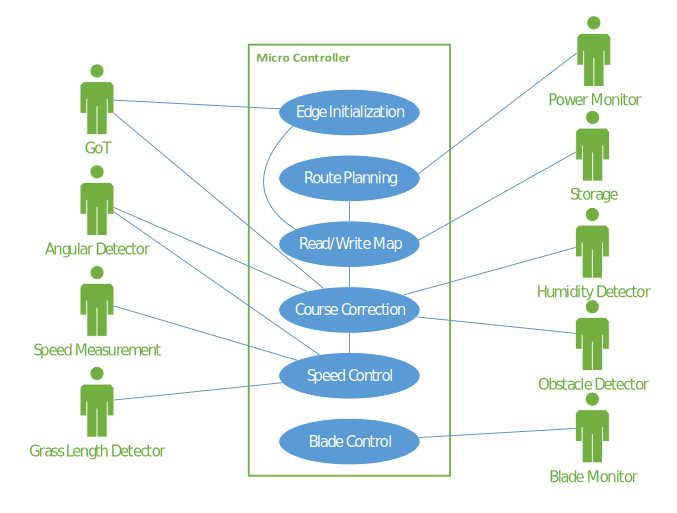
\includegraphics[scale=0.8]{figures/P5UseCase.pdf}
	\caption{Use-Case Diagram}
	\label{fig:usecase}
\end{figure}

\noindent
\newpage

The system, inside the controller, have 6 main functionalities and is affected by 9 different actors.

\subsection{Main Functionalities}

Functionalities are the functions that the system can do. Each Functionality can have more than one function in the system. The functionalities get input from actors and can be in association with other functionalities. 

\textbf{Edge Initialization}:
The \textit{Edge Initialization} gets input from the \textit{GoT} system and is associated with the \textit{Read/Write Map} functionality. The purpose of this function, is to calibrate the system to a new lawn. The function is making a edge map of the lawn. It used it to locate all the areas, where the lawn shall be mowed and where the lawn mower shall not drive. This is done, by manually moving the \textit{GoT} system's transmitter  along the edges of these areas. From the information about all the edges, the edge map is created and saved through the \textit{Read/Write Map} function.

\textbf{Route Planning}:
The \textit{Route Planning} gets input from the \textit{Power Monitor} and is associated with the \textit{Read/Write Map} functionality. The purpose of this function, is to plan the route for the lawn mower. The route is made from the information about where the lawn mower starts, the map of the lawn, which is made in the \textit{Edge Initialization} function. The map is loaded from the \textit{Storage} with the \textit{Read/Write Map} function. It also needs the battery level from the \textit{Power Monitor}. The route has to cover the whole lawn.

\textbf{Read/Write Map}:
The \textit{Read/Write Map} gets input from the \textit{Storage} and is associated with the \textit{Route Planning}, \textit{Course Correction} and the \textit{Edge Initialization} functionalities. This functionality communicates with the storage. In the \textit{Storage} the edge map from the \textit{Edge Initialization} function is saved and loaded from. The route from the \textit{Route Planning} is saved there to. The route is loaded and send to the \textit{Course Correction} functionality, when the system is driving.

\textbf{Course Correction}:
The \textit{Course Correction} gets input from the \textit{GoT} system, the \textit{Humidity Detector}, the \textit{Obstacle Detector} and the \textit{Angular Detector} and is associated with the \textit{Read/Write Map} and the \textit{Speed Control} functionalities. This function measures the surroundings of the lawn mower and makes corrections, in case of disturbances which might otherwise throw it off its route. The function makes the lawn mower stay on the route, which it get from the \textit{Read/Write Map} function, when the route can be followed. The \textit{Course Correction} is the main function behind the regulation of the movement of the lawn mower and sends these regulations to the \textit{Speed Control} function.

\textbf{Speed Control}:
The \textit{Speed Control} gets input from the \textit{Angular Detector}, the \textit{Grass Length Detector} and the \textit{Speed Measurement} and is associated with the \textit{Course Correction} functionality. The function's purpose, is to make sure that the lawn mower smoothly adapts the speed depending on the grass length, to get a more evenly cutting, and the curves of the route. This function controls the drive motor's speed, depending on route and regulation of the current speed.

\textbf{Blade Control}:
The \textit{Blade Control} gets input from the \textit{Blade Monitor}. The function's purpose, is keeping the blade rotational speed the same, to make an evenly cut. With the input from the \textit{Blade Monitor}, the \textit{Blade Control} regulate the speed to be constant.

\subsection{Actors}

A actor is a external system or component, that influence the system with inputs to the functionalities and/or gets output from them.

\textbf{Humidity Detector}:
The \textit{Humidity Detector} is connected to the functionality \textit{Course Correction}. This is a sensor that measures the humidity in the air. The system uses the information about the ambiant humidity level to see, whether it is too high to mow the lawn in or not, since wet grass can not be cut evenly and the cut of grass could damage the equipment. 

\textbf{GoT}:
The \textit{GoT} system is connected to the \textit{Course Correction} and \textit{Edge Initialization} functionalities. This system is used to get the lawn mower's position on the lawn. This position is sent to the controller, which uses the information to guide the lawn mower along its route.

\textbf{Storage}:
The \textit{Storage} is connected to the \textit{Read/Write Map} functionality. It uses a static storage to store the information about the edge map and route, which is made in the \textit{Edge Initialization} and \textit{Route Planning} functionalities. The \textit{Storage} will have the data saved, even if the system is turned off.

\textbf{Obstacle Detector}:
The \textit{Obstacle Detector} is connected to the \textit{Course Correction} functionality. This sensor detects, if there are any objects, which blocks the lawn mower's route. This sensor makes sure, that the lawn mower keeps a distance to any object, like a human or a dog that could interfere with its route.

\textbf{Angular Detector}:
The \textit{Angular Detector} is connected to the \textit{Course Correction} and \textit{Speed Control} functionalities. This sensor measures the angular position and movement of the lawn mower, whether it is intentional movement or if the lawn mower slips. This sensor is used as a feedback, to keep the lawn mower on the route.

\textbf{Grass Length Detector}:
The \textit{Grass Length Detector} is connected to the \textit{Speed Control} functionality. This sensor measure the  grass length, which affects the speed, at which the lawn mower should drive. If the grass is long and that it cuts, the lawn mower has to drive slower, to make sure that it doesn't get stuck in the grass and cut the grass evenly. 

\textbf{Power Monitor}:
The \textit{Power Monitor} is connected to the \textit{Route Planning} functionality. This sensor measures how much power  is left in the battery. This is needed, so that the lawn mower can drive back to its charging station, before the battery is empty.

\textbf{Blade Monitor}:
The \textit{Blade Monitor} is connected to the \textit{Blade Control} functionality. This sensor measures the rotational speed of the blade and send the information back to the \textit{Blade Control}, making a feedback loop.

\textbf{Speed Measurement}:
The \textit{Speed Measurement} is connected to the \textit{Speed Control} functionality. The sensor measure the speed, in which the lawn mower drive with. This information is send to the \textit{Speed Control} as feedback.
\section{Vehicle description}

\subsection{The vehicle in general}

The vehicle is composed of two tracks enveloping 4 wheels plus a gear wheel connected to the differential gear by a chain. The servo controls the steering of the vehicle by braking one track or another, so that the motor only control the absolut speed and not the turning. The differential gear is powered directly by the motor.\\
A Hall sensor is plugged on each gear wheel to control the speed of each belt.\\
A platform of the same size of the vehicle is mounted on the vehicle, to support the PCB, the battery, and the sensors used to control the path of the vehicle.\\

\todo{have to put the dimensions and weight of the vehicle}
\subsection{Hall Sensor}

There are two hall sensors implemented on the vehicle, one on each belt. A hall sensor is a sensor that is activated when exposed to a magnetic field. The sensors are placed beside the front wheels, on which there are four magnets, placed so that there is a quarter of a turn between them. The hall sensor is illustrated on \figref{HallSensor}.

 \begin{figure}[H]
	\centering
	\includegraphics[scale=0.5]{figures/HallSensorSide_Forward_view.pdf}
	\caption{Illustration of the hall sensor.}
	\label{HallSensor}
\end{figure}

The Hall sensor will give a voltage output each time one of the magnets is in front of the hall sensor. This will give a signal each quarter of a turn of the wheel. As the distance between each magnets is not the same, the calculations will be taken for each magnets independently.
Knowing the time a turn of the wheel will take by measuring the time between four outputs, and the distance that the vehicle travels on that time, the speed of the vehicle can be calculated.

When the vehicle is starting to move, the first turn of the wheel can not be used because the calculations are made independently for each magnets. Therefore the speed can only be calculated by the first output of the second turn.\\\\


The two hall sensors are independent for being able to measure each belt when the vehicle turns through braking one track thanks to the servo.
\subsection{Servo}
On the vehicle there is a servo, which is a S3003 by Futaba. \todo{Insert ref to the datasheet}
The servo is used for the steering of the vehicle. The servo controls the steering through breaking one of the belts, in part 3 on \figref{} in \secref{}, and transfer that power over to the other belt, thanks to the differential gear box.

The Servo is controlled by a PWM signal from the arduino card. The received PWM signal is converted into an angle by the servo to control the steering of the belts, as seen on \figref{timeVSangle}.

A mechanical arm is mounted on the servo and connected to the brakes of the tracks. When the servo rotates one way, it triggers the brakes more on one side and stop breaking at the other side, according to the value of the angle sent, through the PWM signal. This way, one of the belt will drive slower and the other belt drive faster, by the help of the differential gear system, which will make the vehicle turn, without decreasing the output power of the system.

\begin{figure}[H]
	\centering
	\includegraphics[scale=0.6]{figures/TimeVSangle.pdf}
	\caption{Convertion from time to angle by the servo}
	\label{timeVSangle}
\end{figure}

The servo reacts linearly to the PWM signal and the cycle of the signal is 30 milliseconds. To get the servo to be in neutral position at 90°, the servo needs a PWM signal of 4.83 \% (a period of 1450 microseconds). For 180°, it is 8.33 \% (a period of 2500 microseconds) and 1.67 \% (a period of 500 microseconds) for 0°. \\\todo{Insert ref to the datasheet}

When the servo brakes on one of the belt, the force, that should be lost in the breaking, is transfer to the other belt, by the differential gear system.
\subsection{Differential gears} \label{sec:Differentialgears}

The differential gear box is located as the first component in the drivetrain, after the connection to the motor (Part 2 on \figref{vehicleDescriptionDriveTrain} in \secref{sec:Vehicledescription}).
When the servo is braking on one of the sides of the drivetrain, the differential gears transfer the rotational energy from this side to the other side. This minimize the lose of energy when braking. The extra speed, sent to the other belt that is not braking, will make the vehicle turn faster compared to a simple brake.

A differential gear system can be seen on \figref{diffGearLight}.

\begin{figure}[H]
	\centering
	\includegraphics[scale=0.7]{figures/diffGearLight}
	\caption{Illustration of a differential gear system. On the left, the resistance on each side is equal, so the spider gear does not rotates. On the right, the resistance on the left side is bigger than the one on the right side, so the spider gear rotates and transfer more rotational energy to the right side. \cite{MechanicalEngineering}}
	\label{diffGearLight}
\end{figure}

The differential gear system contains a ring gear (blue), a spider gear (green), two side gears connected to the rest of the system (red and yellow) and a pinion gear (not shown on picture) connected to the ring gear, that transfer the power from the motor to the system.\\

When the motor is running, the pinion gear transfer a rotational energy to the ring gear. The spider gear, fixed on to the ring gear, begins to rotate around the side gear. If the resistance on both side gears is the same, the same power is needed to rotate the gears. Therefore the spider gear will not rotate around its own axis and apply the same rotational energy to each side gear.\\

When the resistance on both sides is not the same, i.g. if one of the side is being brake on, the spider gear will rotate around is own axis. There is a bigger resistance on one side than on the other, so the side not braking will be easier to rotate. The ring gear and the spider gear are rotating at the same speed around the two side gears, but the spider gear will apply less rotational energy on the braking side than on the other side, because of it own rotation. In the case that the resistance on one side is infinite, as the spider gear is rotating at the same speed that the ring gear, the side gear on the none braking side will therefore rotate twice as fast, with the assumption that there is no loss in the system.\\

For the differential gear system on the vehicle, there is a more complete setup, shown on \figref{diffGearFull}
	%\caption{Illustration of the differential gear system on the vehicle \cite{MechanicalEngineering}}

\begin{minipage}{\linewidth}
      \centering
      \begin{minipage}{0.65\linewidth}
          \begin{figure}[H]
              \includegraphics[width=0.95\textwidth]{figures/diffGearFull}
              \caption{Illustration of the differential gear system on the vehicle \cite{MechanicalEngineering}}
              \label{diffGearFull}
          \end{figure}
      \end{minipage}
      \hspace{0.05\linewidth}
      \begin{minipage}{0.25\linewidth}
      		\begin{enumerate}
      			\item Pinion gear
      			\item Ring gear
      			\item Spider gears
      			\item Side gears
      		\end{enumerate}
      \end{minipage}
  \end{minipage}




%\begin{table} [H]
%\begin{tabular}{p{3cm} p{3cm}}

%\begin{figure}
%	\includegraphics[scale=0.7]{figures/diffGearFull}
%	\label{diffGearFull}
%\end{figure}

%&

%\begin{enumerate}
 % \item Hallo
%\end{enumerate}

%\end{tabular}
%\end{table}




%\begin{figure} [h]
%	\centering
%	\includegraphics[scale=0.7]{figures/diffGearFull}
%	\caption{Illustration of the differential gear system on the vehicle \cite{MechanicalEngineering}}
%	\label{diffGearFull}
%\end{figure}

Instead of only having one spider gear (the green gear on \figref{diffGearLight}) there is two for more reliability and solidity, shown in red on \figref{diffGearFull}. The system works in the same way as with one spider gear, with the pinion gear (1) transfering the power to the ring gear (2). The spider gears (3) fixed on the ring gear rotates the side gears (4) compared to their own resistance.

Now that the vehicle has been presented and its limits analysed, the prototype contraints can be considered to aim the functionnalities needed in this project.

\subsection{Things that maybe should be placed in this section}

When a permanent magnet DC motor is used, the inductor and resistor in the motor causes a time constant, that the PWM time period should be less than:

\begin{flalign}
T &< 2 \cdot \frac{L_a}{R_a} \cdot ln(1-\frac{P}{100})\unit{s}
\end{flalign}

Where P is the duty cycle in percent, and La is the inductance in the motor, and Ra is the resistance in the motor.

\section{Prototype Constraints}
Before the prototype can be established, some considerations have to be made in respect to the time limitations and the main scope of this semester. The aim of the project is to create a functional automated proof of concept lawn mower. The following section includes a brief description of the technology on which the prototype is constructed, along with argumentation for eliminated functionalities.

\subsection{Technology Base}
The technology which has been provided for the prototype is a tracked vehicle, seen on \figref{TrackedVehicle}. The vehicle comes with a brushed DC motor which provides power for rotation of the wheels connected to the belts. Furthermore a servo motor is used to control the ratio of the differential steering, by utilize breaks connected to the wheels. The tracked vehicle includes two hall sensors, one by each belt, which keeps track of the speed, of the belts, by measuring pulses from magnets mounted on the front wheels. The testing will take place in Aalborg University Vicon Room, where the GoT system is installed and calibrated with the appurtenant transmitter, which is mounted on the tracked vehicle during test.

\begin{figure}[H]
	\centering
	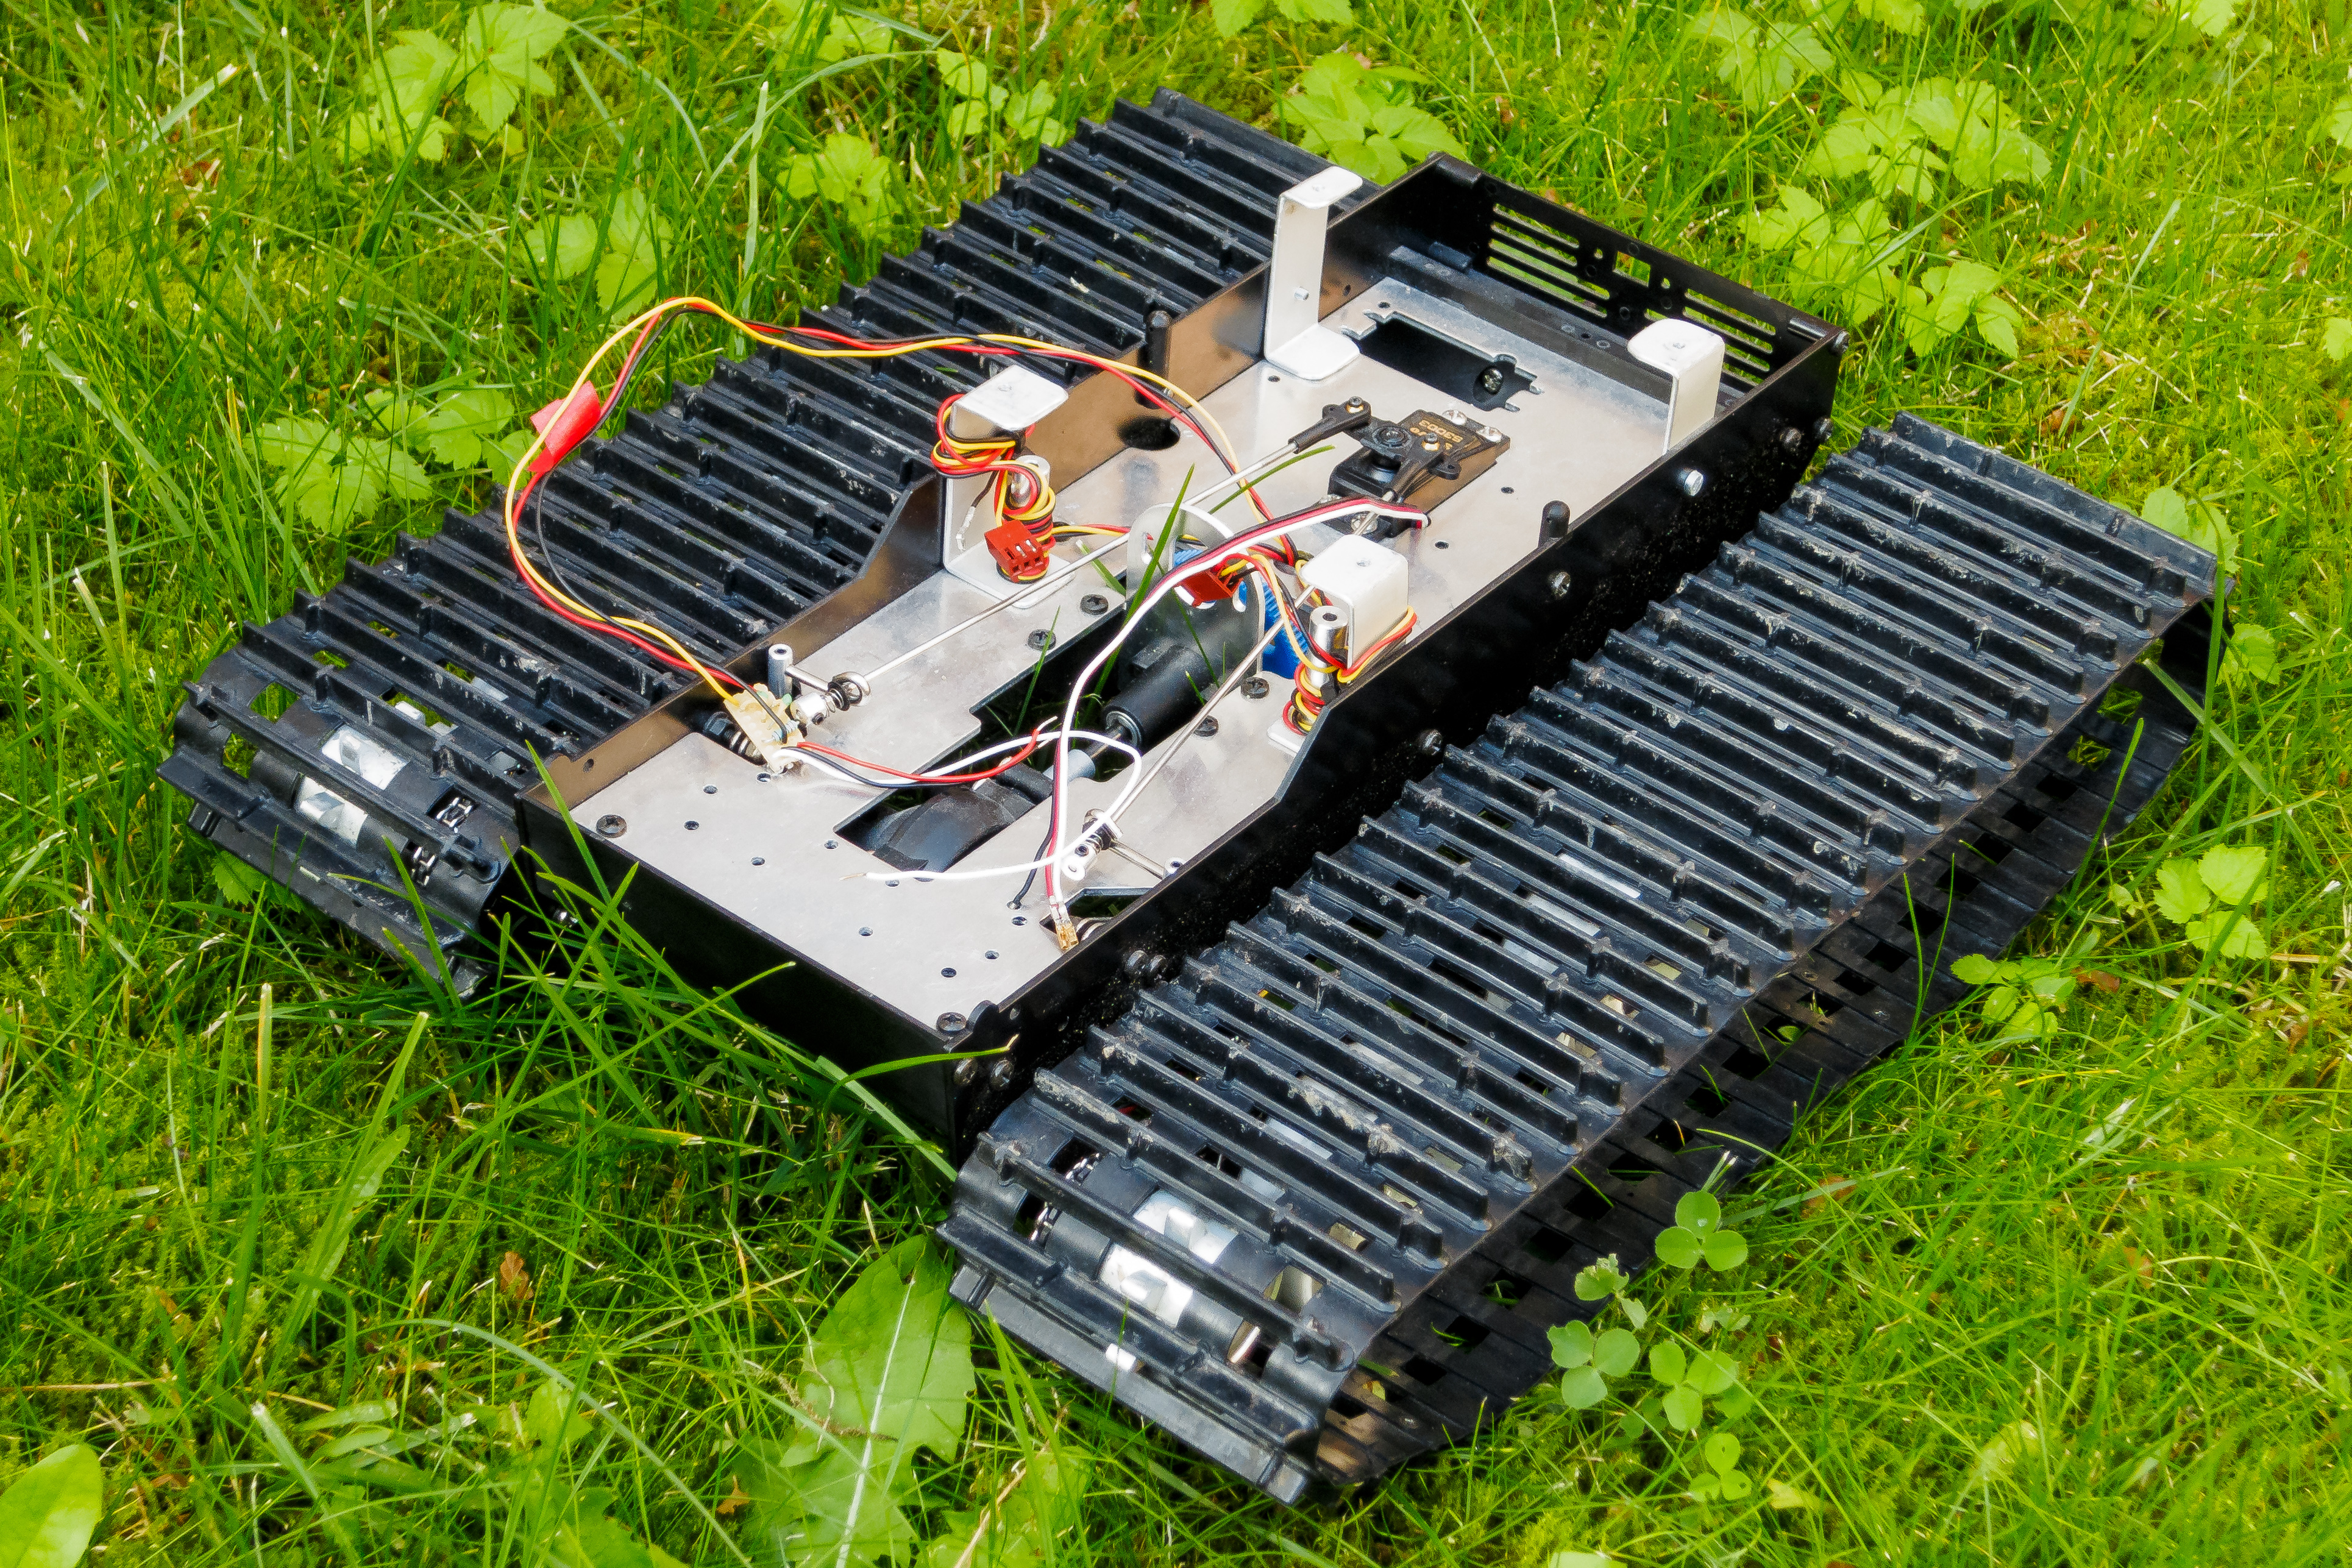
\includegraphics[scale=0.8]{figures/BeltVehicle.jpg}
	\caption{The provided track vehicle}
	\label{TrackedVehicle}
\end{figure}

\todo{datasheet of the vehicle}

\subsection{Grass Length Detection}
Detection of the grass length to control the speed of the lawn mower thus ensuring an evenly cut lawn, is a submodule which can be added at any time. Since it is not fatal for a working system and might even be unnecessary depending on time between each mowing of the lawn, it is decided to exclude this functionality from the initial design.

\subsection{Humidity Sensor}
As the lawn mower is supposed to work outside, it is important to consider that the grass could be humid. Since it is difficult to cut humid grass, a humidity sensor could be used to warn the system of the humidity. Thus the system could go back to the charging station. However, the prototype will only be tested indoor, so this type of sensor will not be necessary in a prototype design.

\subsection{Obstacle Avoidance}
The lawn movers path might not always be clear, e.g. garden tools, tables or moving objects could be in the way. The vehicle should be aware of what is in front of it at any time, to correct its path and get around the obstacle if necessary. To avoid this the sensor could be a pushing button to detect a solid object or an ultrasound detector if the object is fragile.
As the aim of the project is to control the path of the vehicle by using angular positioning sensors, a proximity sensor will not be included. Static objects could be registered on the map to avoid these issues.\\\\
Furthermore the edge mapping functionality will not be included in the project which instead will focus on a quadratic map predefined in the test room.

\subsection{Power Monitoring}
Power monitoring could be implemented by measuring the voltage across the batteries, to ensure that the lawn mower is not running out of power, and to ensure the vehicles calculated route passes the charging station before the power runs too low.
This and the charging station will not be in the prototype, since it is beyond the scope of the project this semester and is not crucial for a working prototype.

\section{Prototype, Interfaces and Submodules} \label{Finalprototype}
%The overall functionalities for the project have been limited, due to time limitations and to focus on the scope of the project. In this project a prototype will therefore be made to show the main functionalities necessary to make an automated vehicle containing principles for lawn mowing.
%In short, the final prototype includes a regulator, which will make it possible to follow a path from A to B. It is able to continue if the wireless connection is lost between the prototype and the GoT system for some duration. Furthermore it is able to plan a route within a given area and store these calculated data points locally, on the vehicle. The rough outline of the design is shown in \figref{fig:systemOverview1} to give an idea of the final prototype setup.

%\begin{figure}[H]
%	\centering
%	\includegraphics[scale=.9]{figures/systemOverview1}
%	\caption{Overview of the system prototype}
%	\label{fig:systemOverview1}
%\end{figure}

%The GoT system provides the vehicle with coordinates, which is utilized in course correction in combination with the map supplied from storage, to follow the route. In course correction lies also control between coordinates given by the GoT system and the storage, this is regulated through use of angular position and movement supplied by the angular sensors. The speed control gets an input from the course correction, the speed given is then held through regulation again using input from angular sensors, in this case specifically acceleration.


%Previously the rough prototype design is presented. To provide a more broad overview of the system, an exploded view of functionalities, their submodules and interfaces is presented in \figref{fig:systemOverview2}.

The overall functionalities for the project have been constrained from the Use-Case \secref{sec:UseCase}, due to time limitations and to focus on the main scope of the semester. A prototype is therefore made to illustrate the main functionalities necessary to make an automated vehicle, containing principles for lawn mowing.

The final prototype includes a regulator, which will make it possible to follow a path from A to B. It is able to continue if the wireless connection is lost between the prototype and the GoT system for some duration. The outline of the design is shown in \figref{fig:systemOverview2} to give an idea of the final prototype setup. In this section, the different functional blocks are put forth along with the interfaces describing the interaction between them.

\begin{figure}[H]
	\centering
	\includegraphics[scale=.9]{figures/systemOverview2}
	\caption{Overview of the software and electronic parts of the system prototype, where the gray modules are hardware and the white are software. The dotted lines are wireless signals while the others are wire signals}
	\label{fig:systemOverview2}
\end{figure}

\subsection{Modules}
In the following all the modules from the system prototype which needs further explanation are described to obtain a basic understanding of the prototype.

%\subsubsection{GoT System}
%%The GoT satellites is placed in the area in which the vehicle needs to operate. These satellites receives information from the vehicle. The time which the vehicles transmitter sends out bursts is received by the GoT master. Furthermore the time which the satellites receives the information send from the vehicles transmitter is transmitted to the GoT master. The GoT master then relays the information received from the vehicle directly to the 
%
%The \textit{GoT Transmitter} placed on the vehicle transmits a signal containing the time at which it send the ultra sound signal to the \textit{GoT Satellites} to the \textit{GoT Master}. The satellites transmit the signal recieved to the master as soon as they recieve it. The master then relays those informations to the \textit{GoT on Computer} that will calculate the position of the car.

\textbf{Computer and Position Decoder:}
The computer handles the calculation of the current position of the vehicle \appref{GoTDescription}. If a packet is disturbed or sent incorrectly it should be possible to detect it, so invalid data is not used by the prototype. It may occur that the coordinates which are sent from the GoT system is out of sensible range, e.g the coordinate transmitted jumps from one location to a location which is unrealistic, for the vehicle to reach in the amount of time between received coordinates. In this event the out of range coordinate should also be disregarded. The computer must compile a package containg the coordinates. The position decoder must be able to decode the send package.

\textbf{Course Correction:}
This module receives the vehicles position from the GoT and the next destination on the path, which is located in the storage. These informations constitutes a path segment on which it is the course correction's task to stay. To accomplish this it receives the angle and the speed of the vehicle, and uses this information to correct its course along the current path segment.

\textbf{Read/Write Map:}
This module handles the writing of coordinates to the nonvolatile storage device, as well as the reading of next desired destination from the stored map.

\textbf{Speed Control:}
This module retrieves the speed of the vehicle from the Get Speed module. This is used, through control, to obtain a steady speed. Furthermore it handles any request of change in speed delivered by the course correction.

%\subsubsection{Edge Map}
%The first time the user will initialise the lawn mower, an \textit{Edge Map} will be created thanks to the GoT system. This edge map will determine the areas that the car is allowed to go or not, in regards of specifications or objects on the lawn.  

%\subsubsection{Route Planning}
%The Route Planning module calculates a route from the points gathered from the Edge Map. The route will be in straight lanes, as in the Bosch Logicut system \secref{roboMowers}, to guarantee that the whole lawn is cut.

%\subsubsection{Angular Sensors}
%The angular position is measured thanks to the \textit{Angular Sensors}, that will send data to the submodule \textit{Get Angle}, in charge to send the angle to the Speed Control and to the Course Correction submodule.

\subsection{Interfaces}
%- To Tom and Rasmus \newline
%In the subsection an explanation of the different interfaces between the modules is made. We have thought about making it like a high layer interface, where we only explain what we need the different modules to give each other. Like one module needs to get the map edge, i.e. coordinates, but since it is this early in the report and it would be more overview by writing map edge rather than coordinates. But as you can see in \figref{fig:systemOverview2} the layers of information are different, one is raw angle data and another time send. Is this okay or should we change something else?
%\indent
%The interfaces of the system is very important when designing each of the adjacent submodules. The existing interfaces as well as the ones presumed are also important in the process of analyzing the system capabilities width focus on requirements of the prototype. Width that in mind follows a brief review of the interfaces between each submodule.
In this section a high layer interface between the modules will be presented. This provides information for designing each of the adjacent submodules individually.

\textbf{8 - Package Containing Position:}
The data communicated from the GoT system to the vehicle contains the last recorded position of the vehicle. This position is presented in the form of an x- and a y-coordinate, which must be included in the data package. Additionally each package must contain decode information for the receiver, including how to separate each package along with error handling.

\textbf{7 \& 4 - Angle/Servo Control Signal \& PWM Signal:}
Course correction will ask the vehicle to turn or make small adjustments of the angle. This angle is realized through the servo motor which breaks on either belt aproprite to the required angle. For the servo to understand the angle the servo driver must translate it into a PWM signal, which makes the servo turn to a specific position for each pulse width.

\textbf{2 \& 1 - Angle \& Raw Angle Data:}

\textbf{6, 5 \& 4 - Desired Speed, Motor Control Signal \& PWM Signal:}

\textbf{11 \& 3 - Hall Sensor Pulses \& Belt Speed:}

\textbf{13 - Route Coordinates:}






%Route Planning, Storage and Read/Write Map Interfaces:
%The Edge Map submodule sends the Map edge to Route Planning, that will send a Route to Read/Write Map. The Route to follow will then be transmited to the Course Correction submodule for a path correction, and to the Storage for saving.

%\textbf{Speed Control Interfaces:}
%The Hall Sensors send Hall sensor pulses to the submodule Get Speed, that will process it to transmit the Belt speed to the Speed Control. A PWM signal containing the new wanted speed will then be sent to the Motor Driver, wich will convert it to the final Motor control signal and sent it to the Drive Motor.
%
%\textbf{Angular Sensors Interfaces:}
%The Angular Sensors will send a Raw angle data to the submodule  Get Angles, that will process it and send the Processed angle data to Course Correction.
%
%\textbf{Course Correction Interfaces:}
%The Course Correction submodule receives the Position and Time from the Wireless Module, the Route to follow from Read/Write Map, and the Processed angle data from Get Angles. With all those information, a decision will be sent to the Speed Control through the Desired speed, and to the Servo Motor with an Angle/servo control signal.

Now that the vehicle had been described and the prototype defined, the modeling of the vehicle can be made.


%---------------------------------------------------------------------------------------------------------------------------\\
%REWRITE THIS SCRAMBLED VERSION OF THE ABOVE TWO SUBSECTIONS \todo{rewrite in the above section and delete these subsections}\\
%---------------------------------------------------------------------------------------------------------------------------
%
%\subsubsection{GoT Satellites, Master and GoT Ultra Sound \& Radio Link}
%\indent
%A number of GoT Satellites are placed in the corners of the area in which the vehicle is to operate. These Satellites receive ultra sound signal from the GoT device placed on the vehicle. The time in which each ultrasound signal is received is passed through a wireless connection from the satellites to the GoT master. The GoT master then pairs this information with the time the ultra sound signal was send from the vehicle which it receives via radio link from the GoT device on the vehicle. After collecting the information, the GoT master sends a calculated position and along with a time stamp to the computer handling GoT.
%
%\subsubsection{Wireless Modules}
%\indent
%%The wireless modules serves the purpose of transmitting the calculated coordinates from the GoT system to the vehicle.
%
%\subsubsection{Edge Map, Route Planning, Read/Write Map and Storage}
%\indent
%%The route planning functionality receives the hard coded edge positions from edge map. Using this information the route is then planned and saved in the storage through the read/write map functionality.
%
%\subsubsection{Gyro, Accelerometer, Magnetometer, Speed Control and Course Correction}
%\indent
%%Gyro along with magnetometer is used for angular position of the vehicle. This is passed to the course correction through the get angle functionality. Here it is used as to correct the orientation of the vehicle on its path. The accelerometer also channels through the get angle functionality. The angular acceleration is then used for correction of the speed.
%
%\subsubsection{Hall Sensor}
%\indent
%%The speed control also receives input from the hall sensors through the get speed functionality, where the inputs from the hall sensors are translated to speed of the vehicle's belts. This information is then used in speed control to regulate the speed.
%
%\subsubsection{Servo Motor}
%\indent
%%The servo motor receives an angle/servo control signal from course correction. This angle equals a given amount of breaking on either of the two belts, which then through the differential gearing translate into steering and thus correction of the course of the vehicle.
%
%\subsubsection{Motor Driver and Drive Motor}
%\indent
%%The drive motor takes a motor control signal from the motor driver provided by the speed control. The control signal from speed control is a PWM signal.



%---------- Chapter 3 ----------------------------------------
\chapter{Modeling of the Vehicle}\label{cha:ModelOfVehicle}

The prototype model contains software, hardware and mechanical components. Software and hardware components are easy to change and to model after how the rest of the system is made and shall run. The vehicle, which is a mechanical plant, is provided to this project and therefore not changeable. This means that requirements about how the system should react, described in \secref{sec:Vehicledescription}, apply only for elements of the system that are external to the plant. In this chapter, a model of the vehicle is made to describe the power transfer from both the motor's and servomotor's rotational energy to the movement of the vehicle. Once, this model is established, it is possible to measure its output and apply a control on it, see \chapref{cha:ControlOfTheVehicle}.


\begin{figure}[H]
	\centering
	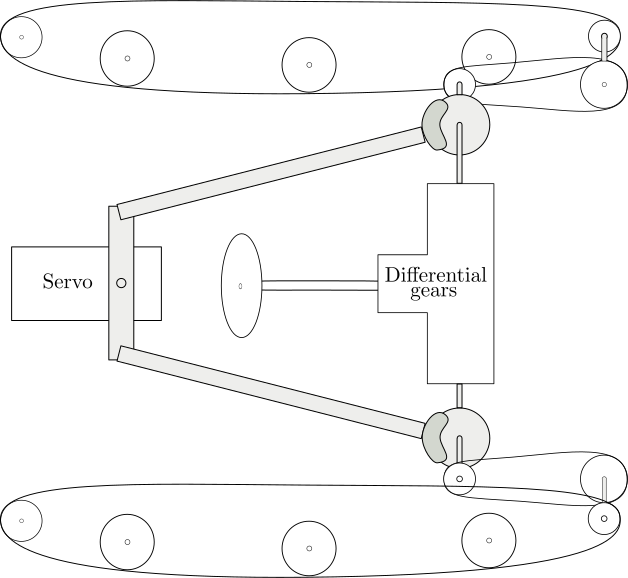
\includegraphics[scale=0.6]{figures/completeMechanical.pdf}
	\caption{A mechanical diagram of the vehicle}
	\label{fig:completeMechanicalDiagram}
\end{figure}

The \figref{fig:completeMechanicalDiagram} shows both the drivetrain and steering mechanisms on the given vehicle. It is possible to identify and separate these two sub-systems. The driving part allows the vehicle to run and comprises the motor, all the gears that make the belts turn and the belts themselves. On the other hand, the steering part is made of the servomotor which acts on two shafts and breaks one or the other belt, as stated in \secref{sec:Vehicledescription}. In the next sections, the drivetrain, which allows the vehicle to run, and the steering part, which allows the vehicle to turn, are modelled separately, and eventually recombined into a single model.
\section{Velocity Model of the Vehicle}
In this section the \textit{Vehicle} block in \chapref{cha:ModelOfVehicle} \figref{fig:StartTotalModelsystem} is opened up and modelled regarding the velocity of the vehicle. In \figref{fig:Velocitymodelplantopen} the opening of the \textit{Vehicle} block is illustrated.

\begin{figure}[H]
	\centering
	\includegraphics[scale=0.6]{figures/plantopen.pdf}
	\caption{The \textit{Vehicle} block in \chapref{cha:ModelOfVehicle} \figref{fig:StartTotalModelsystem} is opened up and illustrated in more detail}
	\label{fig:Velocitymodelplantopen}
\end{figure}

The velocity model of the \textit{vehicle} has been split up into a motor and a drivetrain section. The motor receives an input from the controller regulating its supplied voltage. the motor then delivers a rotational force as an output to the drivetrain. The drivetrain then generates the actual speed as the output of the \textit{Vehicle} block. as well as supplying the motor with an angular velocity which is dependent on the total inertia of the system, and thereby insures that the motor is affected by its load. The two sections, the motor and drivetrain, is generated by only considering the parameters affecting the vehicle when the vehicle is driving in a straight line. Thus, excluding the differential steering and thereby only modelling the system when the wheels have the exactly same velocity.

In the following subsection the motor will be modelled.
\subsection{Motor modelling}
A model of a motor consist of both a mechanical and an electrical section, due to the electrical current, $i_a(t)$, converting into a rotational force called torque, $\tau_m$. Therefore a model of the mechanical and the electrical system is produced. The electrical model provides the motors torque and the mechanical model from the motor provides what contributions the motor delivers to the drivetrain, see \secref{DriveTrain}.

\subsubsection{Electrical model}
The output from the motors electrical model is torque, $\tau_m$. To obtain the torque, the formula for translating the electrical current, $i_a$, to torque is utilized:

\begin{flalign}\centering
  \tau_m(t) = K_t \cdot i_a(t) %\unit{\volt}
  \label{equ:motortorque}
\end{flalign}
\hspace{6mm} Where:\\
\begin{tabular}{p{1cm}ll}
& $\tau_m$ & is the rotational force torque [$N \cdot m$] \\
& $i_a(t)$ & is the electrical closed loop current [$A$]\\
& $K_t$ & is the torque constant [$\frac{N \cdot m}{A}$] \\
\end{tabular}

An expression for the current, $i_a$, is required to derive a model for the electrical system. In \figref{fig:electricaldiagrammotor} an electrical diagram of the motor is displayed.

\begin{figure}[H]
\centering
	\begin{circuitikz}[american voltages]
		\draw
		
		% electromotive force 
		(0,0) to [short] (6,0)
		%to [sV, l=$e_b$] (6,2) %  voltage
		(6,0) to [V, l=$e_b$] (6,3)
		%to node[short]{}(6,2)

		%to node[short]{}(0,0)		 
		(0,0) to [V, l=$V_m$] (0,3) %  voltage

		
		%to [R, l=$Z_G$] (3,3) % generator impedance
		
		(0,3) to [R, l_=$R_a$, i>_=$i_a$] (3,3)	
		
		to [L, l_=$L_a$] (6,3); 
	\end{circuitikz}
  \caption{A electrical diagram of the motor}
  \label{fig:electricaldiagrammotor}
\end{figure}

By using Kirchoffs voltage law on the closed loop, seen in \figref{fig:MotorElectric}, an expression including $i_a$ can be derived:

\begin{flalign}\centering
V_a(t) = R_a \cdot i_a(t) + L_a \cdot \frac{di_a}{dt} + e_b 
\label{MotorClosedLoop}
\end{flalign}
\hspace{6mm} Where:\\
\begin{tabular}{p{1cm}ll}
& $V_a(t)$ & is the supply voltage [$V$] \\
& $R_a$ & is the internal resistance in the motor [$\Omega$]\\
& $L_a$ & is the inductance in the motor [$H$] \\
& $e_b$ & is the electromotive force, also called EMF [$\V$] \\
\end{tabular}

The electromotive force, $e_b$, is equivalent to:

\begin{flalign}\centering
e_b = K_e \cdot \dot{\theta}_m(t) 
\end{flalign}
\hspace{6mm} Where:\\
\begin{tabular}{p{1cm}ll}
& $K_e$ & is the electromotive constant [$Wb$] \\
& $\dot{\theta}_m$ & is the angular velocity in the motor [$\frac{rad}{s}$] \\
\end{tabular}

The equivalent for the electromotive force is substituted into \eqref{MotorClosedLoop}.

\begin{flalign}\centering
V_a(t) = R_a \cdot i_a(t) + L_a \cdot \frac{di_a}{dt} + K_e \cdot \dot{\theta}_m(t)
\end{flalign}

The Laplace transform is applied to the derived equation:

\begin{flalign}\centering
V_a(s) = R_a \cdot i_a(s) + L_a \cdot s \cdot i_a(s) + K_e \cdot \omega_m(s) 
\end{flalign}

The equation is solved for $i_a$:

\begin{flalign}\centering
i_a(s) = \frac{V_a(s) - K_e \cdot \omega_m(s)}{sL_a + R_a} 
\end{flalign}

By substituting the derived equation for $i_a$ into \eqref{equ:motortorque}, a new expression for the motors torque is derived. 

\begin{flalign}\centering
  \tau_m = K_t \cdot i_a(s) = K_t \cdot \frac{V_a(s) - K_e \cdot \omega_m(s)}{sL_a + R_a}  %\unit{\volt}
  \label{eq:Totaltorquewithcurrentexpression}
\end{flalign}

A equation for the electrical model relative to the motors torque has been derived.

\subsubsection{Mechanical model}
A mechanical model is formed to analyse the forces and moments affecting the mechanical system, and to see how the system reacts to stimuli.

Newtons second law of motion for rotational systems yields:

\begin{flalign}\centering
\tau_m(t) = J_m \cdot \ddot{\theta}_m(t)
\label{eq:mechanicalmodel}
\end{flalign}
\hspace{6mm} Where:\\
\begin{tabular}{p{1cm}ll}
& $J_m$ & is the motors inertia [$kg*m^2 $] \\
& $\ddot{\theta}_m$ & is the angular acceleration in the motor [$\frac{rad}{s^2}$] \\
\end{tabular}

This law is applied to the mechanical model and visualized in \figref{fig:MotorMechanicalModel}. Furthermore it is necessary to consider the friction affecting the rotation of the motor when it is spinning. The friction is in the opposite direction of the applied rotational force torque, see \figref{fig:MotorMechanicalModel}.

\begin{figure}[H]
	\centering
	\includegraphics[scale=0.8]{figures/MotorMechanicalModel.pdf}
	\caption{A free body diagram of the motor}
	\label{fig:MotorMechanicalModel}
\end{figure}

From the figure an equation for the mechanical model can be derived.

\begin{flalign}\centering
\tau_m(t) = J_m \cdot \ddot{\theta}_m(t) + B \cdot \dot{\theta}_m(t)
\end{flalign}

The equation is transferred into the frequency domain using the Laplace transform: 

\begin{flalign}\centering
\tau(s) = J_m(s) \cdot \omega \cdot s + B \cdot \omega_m
\label{eq:ThetadotforBlock}
\end{flalign}

The mechanical model of the motor has be derived. Next step is to make block representation of the system. 

\subsubsection{Block representation}

\eqref{eq:Totaltorquewithcurrentexpression} delivers the information needed to make a visual representation of the motor model. The input is the supply voltage, $V_a(s)$ delivered to the motor and the output is the required torque, $\tau_m$, see \figref{fig:motormodelBlock}. The block representation of the system can be used, when the system is to be simulated.

\begin{figure}[H]
	\centering
	\includegraphics[scale=0.9]{figures/motormodelBlock.pdf}
	\caption{A block representation of the motor, with a voltage, $V_m(s)$, as the input and a rotational force, $\tau_m(s)$, as the output.}
	\label{fig:motormodelBlock}
\end{figure}

The angular velocity received is dependent on the total inertia of the system, and is necessary to insure the motor is affect by the load.

A model of the electrical and mechanical part has been formed and a block representation of the motors applied voltage and generated torque has been given. Next step is to model the drivetrain, which connects to the motor through the motor shaft.
\subsection{Drivetrain}\label{Drivetrain}

%% INTRODUCTION %%
The drivetrain translates the torque $\tau_m$, given by the motor, into the actual movement of the vehicle. The model of the drivetrain illustrates the relation between the applied torque, $\tau_m$, and the velocity of the vehicle. The velocity model of the drivetrain is created by only considering when the vehicle's trajectory follows a straight line.\\\\
%
The modelling of the drivetrain is limited to only model parts of the total drivetrain system, to make it more manageable and with a focus on giving a rough approximation.
%% SSSECTION : BLACK BOX MODEL %%
\subsubsection{Black Box Model}\label{BlackBoxModel}
To get a rough approximation of how the drivetrain works, a blackboxed model is used. The blackbox in the model is placed between box 1 and box 4 seen in \chapref{VehicleDescription} \figref{vehicleDescriptionDriveTrain}. The gear, $G_m$, connected to the motor shaft, is connected to the gear ,$G_d$, which represents the gears and shaft that has been black boxed and the drive-wheel, see \figref{fig:DrivetrainMechanicalModel}. The number of teeth on the gear, $G_d$, is set to the total gear ratio of the black box.

\begin{figure}[H]
	\centering
	\includegraphics[scale=0.8]{figures/mechanicalDrawingSystem.pdf}
	\caption{A rough mechanical diagram of the drivetrain}
	\label{fig:DrivetrainMechanicalModel}
\end{figure}
\todo{Add notations to the diagram and create free body diagrams of belt and black box parts}

% APPLICATION OF NEWTON'S SECOND LAW %

\begin{figure}[H]
	\centering
	\includegraphics[scale=0.8]{figures/freeBodyMotorGear.pdf}
	\caption{A free body diagram of the motor gear}
	\label{fig:MotorGearFreeBodyDiagram}
\end{figure}

\begin{figure}[H]
	\centering
	\includegraphics[scale=0.8]{figures/freeBodyDrive.pdf}
	\caption{A free body diagram of the `black box' gear}
	\label{fig:BlackBoxGearFreeBodyDiagram}
\end{figure}

The \eqref{eq:mechaUnloadedMotor} is extended with the contribution of the load which is the whole drivetrain. Therefore, from \figref{fig:MotorGearFreeBodyDiagram} and Newton's second law appplied to rotational systems, the following equation can be extracted:
\begin{flalign}\centering
J_m \cdot \dot{\omega}_m(t) = \tau_m(t) - B_m \cdot \omega_m(t) - N_m \cdot f_c(t) 
\label{eq:MotorGearNewtonSecLaw}
\end{flalign}
\hspace{6mm} Where:\\
\begin{tabular}{p{1cm}ll}
& $J_m$ 			      & is the motor's inertia [$kg \cdot m^2$] \\
& $\omega_m$        & is the angular velocity of the motor [$rad \cdot s^{-1}$] \\
& $\dot{\omega}_m$ 	& is the angular acceleration of the motor [$rad \cdot s^{-2}$] \\
& $\tau_m$ 		     	& is the torque delivered by the motor [$N \cdot m$] \\
& $B_m$             & is the coefficient of the friction happening inside the motor [$N \cdot m \cdot s \cdot rad^{-1}$] \\
& $N_m$             & is the number of teeth of the motor gear $G_m$ [$number\ of\ teeths$] \\
& $f_c$             & is the coefficient of the contact force between $G_m$ and $G_d$ [$N \cdot m \cdot number\ of\ teeths^{-1}$]
\end{tabular}

The equation for \figref{fig:BlackBoxGearFreeBodyDiagram} is obtained the same way:
\begin{flalign}\centering
J_d \cdot \dot{\omega}_d(t) = N_d \cdot f_c(t) - N_d \cdot f_b(t)
\label{eq:BlackBoxGearNewtonSecLaw}
\end{flalign}
\hspace{6mm} Where:\\
\begin{tabular}{p{1cm}ll}
& $J_d$ 			      & is the `black box' gear inertia [$kg \cdot m^2$] \\
& $\omega_d$        & is the angular velocity of the `black box' gear [$rad \cdot s^{-1}$] \\
& $\dot{\omega}_d$ 	& is the angular acceleration of the `black box' gear [$rad \cdot s^{-2}$] \\
& $N_d$ 		     		& is the number of teeth on the `black box' gear [$number\ of\ teeth$] \\
& $f_b$             & is the coefficient of the contact force between $G_d$ and the belt [$N \cdot m \cdot number\ of\ teeths^{-1}$] \\
\end{tabular}

%% SSSECTION : BELT MODEL %%
\subsubsection{Belt Model}\label{BeltModel}

\begin{figure}[H]
	\centering
	\includegraphics[scale=0.8]{figures/mechanicalDrawingBelt.pdf}
	\caption{A mechanical diagram of the belt part}
	\label{fig:BeltMechanicalDiagram}
\end{figure}

\begin{figure}[H]
	\centering
	\includegraphics[scale=0.8]{figures/freeBodyBelt.pdf}
	\caption{A free body diagram of the belt driven mass}
	\label{fig:BeltFreeBodyDiagram}
\end{figure}

From \figref{fig:BeltFreeBodyDiagram}, the mechanical equation of the belt system on \figref{fig:BeltFreeBodyDiagram} is found to be:
\begin{flalign}\centering
M \cdot \dot{v}(t) = r_t \cdot f_b(t) - B_{sys} \cdot v(t)
\label{eq:BeltMassNewtonSecLaw}
\end{flalign}
\hspace{6mm} Where:\\
\begin{tabular}{p{1cm}ll}
& $M$ 			  & is the vehicle's total weight [$kg$] \\
& $v$        	& is the linear velocity of the behicle [$m \cdot s^{-1}$] \\
& $\dot{v}$ 	& is the linear acceleration of the vehicle [$m \cdot s^{-2}$] \\
& $r_t$ 		  & is the translational coefficient between the last gear and the belt [$m \cdot number\ of\ teeths^{-1}$] \\
& $B_{sys}$   & is the coefficient of the friction happening throughout the gears [$N \cdot s \cdot rad^{-1}$] \\
\end{tabular}

The assembling of a model for the drivetrain is made from these separate mechanical equations.

% SSSECTION : ASSEMBLING OF THE DIFFERENT EQUATIONS %
\subsubsection{Drivetrain modeling}\label{DrivetrainModeling}
The combination of \eqref{eq:MotorGearNewtonSecLaw}, \eqref{eq:BlackBoxGearNewtonSecLaw} and \eqref{eq:BeltMassNewtonSecLaw} makes it possible to get the linear velocity of the vehicle $v$ out of the torque $\tau_m$ given by the motor. Indeed, it is possible to link these equations throughout the contact force coefficients $f_c$ and $f_b$.\\\\
%
Taking the Laplace-transform of these equations helps arranging them and eventually, to find a transfer function from $\tau_m(s)$ to $V(s)$ :
%
\begin{flalign}\centering
J_m \cdot s \cdot \omega_m(s) = \tau_m(s) - B_m \cdot \omega_m(s) - N_m \cdot F_c(s) 
\label{eq:MotorGearNewtonSecLawLaplace}
\end{flalign}
%
\begin{flalign}\centering
J_d \cdot s \cdot \omega_d(s) = N_d \cdot F_c(s) - N_d \cdot F_b(s)
\label{eq:BlackBoxGearNewtonSecLawLaplace}
\end{flalign}
%
\begin{flalign}\centering
M \cdot s \cdot V(s) = r_t \cdot F_b(s) - B_{sys} \cdot V(s)
\label{eq:BeltMassNewtonSecLawLaplace}
\end{flalign}
%
By finding the expressions for $F_b$ from \eqref{eq:BeltMassNewtonSecLawLaplace} and then $F_c$ from \eqref{eq:BlackBoxGearNewtonSecLawLaplace}, it is then possible to insert $F_b$ expression into $F_c$'s and the latter into \eqref{eq:MotorGearNewtonSecLawLaplace}.
%
\begin{flalign}\centering
r_t \cdot F_b(s) =  M \cdot s \cdot V(s) - B_{sys} \cdot V(s) 
\label{eq:BeltContactForceLaplace}
\end{flalign} \todo{Get the second implication to be on the next line}
%
\begin{flalign}\centering
F_b(s) =  \frac{M \cdot s \cdot V(s) - B_{sys} \cdot V(s)}{r_t}
\label{eq:BeltContactForceLaplace}
\end{flalign} \todo{Get the second implication to be on the next line}

And $F_c$ is found this way from \eqref{eq:BlackBoxGearNewtonSecLawLaplace}:
\begin{flalign}\centering
N_d \cdot F_c(s) = J_d \cdot s \cdot \omega_d(s) + N_d \cdot F_b(s) 
\end{flalign}
\begin{flalign}\centering
F_c(s) =  \frac{J_d \cdot s \cdot \omega_d(s) + N_d \cdot F_b(s)}{N_d} =  \frac{J_d \cdot s}{N_d} \cdot \omega_d(s) + F_b(s)
\label{eq:GearsContactForceLaplace}
\end{flalign}

\todo{Get the steps to be on different lines}
%
Moreover, the relation of velocity for two gears $G_m$ and $G_d$ in contact is given by:
\begin{flalign}\centering
N_m \cdot \omega_m = N_d \cdot \omega_d, 
\label{eq:GearsVelocityRelation}
\end{flalign}

which is equivalent to :
\begin{flalign}\centering
\omega_m = \frac{N_d}{N_m} \cdot \omega_d \xRightarrow{\mathcal{L}} \omega_m(s) = \frac{N_d}{N_m} \cdot \omega_d(s).
\label{eq:BlackBoxGearNewtonSecLaw}
\end{flalign}
%
The same principle is applied from the angular velocity $\omega_d$ to the translational velocity $V$:
\begin{flalign}\centering
v(t) = r_t \cdot \omega_d(t) = r_t \cdot \frac{N_m}{N_d} \cdot \omega_m(t) \xRightarrow{} \omega_m(t) = \frac{N_d}{N_m \cdot r_t} \cdot v(t)
\label{eq:BlackBoxGearNewtonLaplaceNew}
\end{flalign}
Again, the Laplace transform is used to manipulate equations more easily:
\begin{flalign}\centering
\omega_m(s) = \frac{N_d}{N_m \cdot r_t} \cdot V(s).
\label{eq:BlackBoxGearNewtonLaplaceNew}
\end{flalign}

It is now possible to replace $\omega_d$ and $F_b$ in \eqref{eq:GearsContactForceLaplace}:
\begin{flalign}\centering
F_c(s) =  \frac{J_d \cdot s}{N_d} \cdot \frac{1}{r_t} \cdot V(s) + V(s) \cdot \left[\frac{M \cdot s + B_{sys}}{r_t}\right] = V(s) \cdot \left[\frac{J_d \cdot s}{r_t \cdot N_d} + \frac{M \cdot s + B_{sys}}{r_t} \right].
\label{eq:GearsContactForceLaplaceNew}
\end{flalign}

And the desired relation between the motor torque and the linear velocity is finally obtained :
\begin{flalign}\centering
\tau_m(s) = J_m \cdot \frac{N_d}{N_m \cdot r_t} \cdot V(s) \cdot s + B_m \cdot \frac{N_d}{N_m \cdot r_t} \cdot V(s) + N_m \cdot \left[\frac{J_d \cdot s}{r_t \cdot N_d} + \frac{M \cdot s + B_{sys}}{r_t} \right] \cdot V(s) = V(s) \cdot \frac{1}{r_t} \cdot \left[\frac{J_m \cdot N_d}{N_m} \cdot s + N_m \cdot J_d \cdot s + M \cdot s + N_m \cdot B_{sys} + B_m \cdot \frac{N_d}{N_m} \right]
\end{flalign}

Therefore, the transfer function from $\tau_m$ to $V$ is :
\begin{flalign}\centering
\frac{V(s)}{\tau_m(s)} = \frac{r_t}{\left[\frac{J_m \cdot N_d}{N_m} + N_m \cdot J_d + M\right] \cdot s + \left[B_{sys} \cdot N_m + B_m \cdot \frac{N_d}{N_m} \right]}
\label{eq:TransferFunctionTorqueToVelocity}
\end{flalign}

Eventually, it is possible to draw a block diagram for the drivetrain, from the motor torque to the vehicle's velocity with \eqref{eq:TransferFunctionTorqueToVelocity} and also back to the angular velocity with \eqref{eq:BlackBoxGearNewtonLaplaceNew}, see \figref{fig:BeltFreeBodyDiagram}.

\begin{figure}[H]
	\centering
	\includegraphics[scale=0.8]{figures/blockDiagramDrivetrain.pdf}
	\caption{A block diagram of the drivetrain}
	\label{fig:BlockDiagramDrivetrain}
\end{figure}

\subsection{Verification of the Velocity Model}
In the former section a simplified first order model of the vehicle's velocity model was established. To ensure the approximation is a reliable model of the system, it is compared to a measured step-response of the vehicle. However, the simulation uses a first order model as described in the previous section, the gain, found in \appref{app:gainTest} and the time constant, found in \appref{app:inertiaTest}, is used as the first orders parameters. In \figref{SimulationIRLsteprespons2} the simulated model's step-response and the measured step-response of the vehicle is illustrated. 
%
\begin{figure}[H]
  \centering
 	%Trim margins @:   left        bottom       right       top
 	\adjustbox{ trim = {.15\width} {.30\height} {.15\width} {.30\height}, clip }
  {
    \includegraphics[width=1.4\textwidth]{figures/SimulationIRLsteprespons2.pdf}
  }
  \caption{A plot illustrating a simulated step-response of the approximated velocity model (the blue line) and a measured step-response of the vehicle (the red line).}
  \label{SimulationIRLsteprespons2}
\end{figure}
%
In \figref{SimulationIRLsteprespons2} the red line is the measured data from the vehicle's step-response. To ensure enough data points is registered by the Hall sensor, when performing the step-response of the vehicle, the vehicle is set to drive at \si{1\ m\cdot s^{-1}} at the start of the test. The vehicle preserves this velocity continuously for three seconds, before the vehicle is set to drive at its maximum velocity. The simulation (the blue line) is set to have the same milestones as the measured step-response of the vehicle. Furthermore it can be seen in \figref{SimulationIRLsteprespons2} that the simulation starts before zero, this is due to rounding errors in simulated transfer-function, which is disregarded.

The occurrence of stiction in the start of the simulation and measured step-response, has been eliminated to a certain extent, which makes it insignificant. Furthermore, even though the vehicle is moving at a velocity of $0$ \si{m \cdot s^{-1}}, the velocity is registered to be $0,04$ \si{m \cdot s^{-1}}, see why in \secref{sec:hallFiltering}. 

The little bump in the beginning of the measured step-response, the red line, is caused by the lag of the Hall sensors. This is, however, disregarded. Additionally, the ripples seen on the measured step-response, when the vehicle is at its maximum velocity, could be caused by different kinds of noise factors, e.g:

\begin{itemize}
\item Uneven belts
\item Uneven floor
\item Belts slipping on the floor
\item Wear and tear on the internal gears
\end{itemize}

The data from the simulated and measured step-response illustrated in \figref{SimulationIRLsteprespons2}, when compared is very similar, except for the bump and ripple on the measured data. Besides these two elements the approximated velocity model is sufficient.
\section{Steering Model of the Vehicle}\label{sec:SteeringModel}
\todo{rewrite}The following section will describe and model the steering of the vehicle. The relationship between the vehicle's speed, the angle of the servo, the brakes, and the actual steering of the vehicle will be examined. A overview of the braking system can be seen in \figref{steeringMechanical}.

 \begin{figure}[H]
 	\centering
 	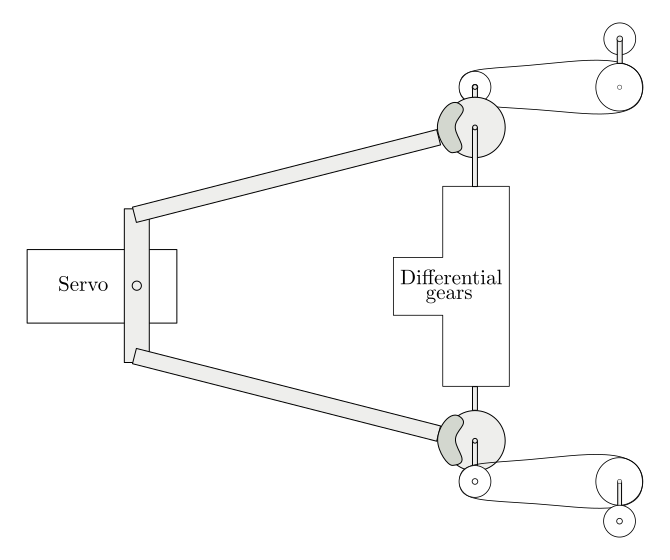
\includegraphics[scale=0.6]{figures/steeringMechanical.pdf}
 	\caption{Mechanical drawing of the steering}
 	\label{steeringMechanical}
 \end{figure}

When the servo turns one way, it push the brake pads on the brake disc, to add a friction. The differential gears will transfer the power from one belt to the other if one brake is triggered.

\subsection{Steering Parameters}
As the steering system contains many moving parts, it would be advantageous to start with a simple model, verifying it, and iterate until it is satisfactory. 

The first model considered can be seen on \figref{basicSteering}.

\begin{figure}[H]
	\centering
	\includegraphics[width=0.8\textwidth]{figures/basic_steering_model.jpg}
	\caption{A basic steering model}
	\label{basicSteering}
\end{figure}
 
As described in \secref{Servo}, the angle of the servo is proportional to a pulse width modulated signal on it's control input. The pulse width is therefore chosen as the input in this model. This is multiplied by a constant, $\text{K}_\text{s}$, which translates the pulse width to an angle of the servo.
If the velocity of the vehicle is assumed constant, the rate of change of the direction must be a function of the servo angle, and a constant, $\text{K}_\text{c}$, representing the speed of the vehicle.
The rate of change is integrated over time, resulting in a direction. 

As the vehicle has to follow a predetermined route, a direction alone is not enough. As seen on \figref{SteeringDeviation}, any change of direction caused by a disturbance, will cause a deviation from the planned line from A to B.

\begin{figure}[H]
	\centering
	\includegraphics[width=0.8\textwidth]{figures/steering_deviation.jpg}
	\caption{Consequence of using directional control alone}
	\label{SteeringDeviation}
\end{figure}

How large the deviation will be must depend on the erroneous angle, the speed, and the time it takes to correct the error. Assuming the speed is constant, the error can be described as an integration of the error angle over time.


Second or first order, if it is second the black box should be expanded, if it is first there is no need because then we have all the parameters from the test.
 
\begin{figure}[H]
	\centering
	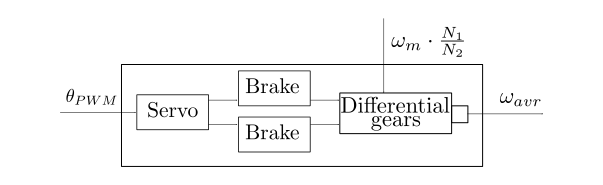
\includegraphics[scale=1]{figures/steeringDiagramBlackBox.pdf}
	\caption{A diagram showing the black box}
	\label{steeringDiagramBlackBox}
\end{figure}
 
%  appendix
 
% show that it's a first order system\\
% then integrator\\
% then is linear(multiples values) the speed of turning at different PWM angle of the servo?


%%% Part 2 %%%
\part{Design \& implementation}

%%% Part 3 %%%
\part{Test \& conclusion}


%%% Setup for Appendix and Bibliography %%%
\bookmarksetup{startatroot} %this is it
\addtocontents{toc}{\bigskip} %perhaps as well
\newpage
\fancyhead[RO]{\color{aaublue}\small Appendix \nouppercase\rightmark} %even page - chapter title
\fancyhead[LE]{\color{aaublue}\small Appendix \nouppercase\rightmark} %uneven page - section title
\fancyhead[RE,LO]{}
\titleformat{\section}[hang]{\Large\bfseries}{\thesection\hsp\textcolor{aaublue}{|}\hsp}{0pt}{\Large\bfseries}
\renewcommand{\thesection}{\Alph{section}}
\setcounter{section}{0}

%%% Appendix %%%
\chapter*{Appendix}
\addcontentsline{toc}{chapter}{Appendix}

%---------- Appendix A ---------------------------------------- GoT Description
\section{The Games on Track GT-position system}
\label{GoTDescription}
The Games on Track GT-Position system, shortened GoT, is a position system which uses radio-waves and ultrasound to locate the object. The system is build up by three types of hardware components: the transmitter, the satellites and the master, see \figref{GoTSystem}. The transmitter and the satellites send the information in all directions, with a 360 degree signal.\\
The GoT System does not work if the transmitter is not close enough from the satellites or if there is some interference by another signal or by an object between them and therefore can not communicate with the satellites.

\begin{figure}[H]
	\centering
	\includegraphics[scale=0.6]{figures/GoT_description.pdf}
	\caption{Overview of the GoT system}
	\label{GoTSystem}
\end{figure}

\subsubsection{Transmitter}
The transmitter component is placed on the object which needs to be located. The transmitter sends an ultrasound burst out containing his id that the satellites are intended to receive. The time at which each ultrasound bursts are sent from the transmitter to the satellites is transmitted by radio waves to the master. There is send an ultra sound burst each tenth of a second, giving a sampling frequency of 10 Hz.\\ 
The transmitter component runs on 2 AA-batteries and therefore does not need an external power-source.\\

\subsubsection{Satellites}
The satellites components are placed around the area where the object, with the transmitter on it, has to be located. The satellites assignment is to search for the ultrasound waves, which the transmitter is emitting, and send a radio wave signal to the master as soon as they receive the burst.
To be able to calculate the exact position of the transmitter and then the object, a minimum of three satellites is necessary. However, more can be added to the system for more reliability or to cover a larger area. To work at a high efficiency, they should be placed at 1 to 2 meters apart and not on a single line. But to cover a bigger area, they can be placed up to a distance of 5 meters between them, although this would affect the measurement and thereby make it less reliable. Each satellite have a maximum range of 8 meters and the three satellites should be placed in each others reach. The satellites need between 14 to 20 volt DC. Thus, making the satellites able to be powered through a computer charger or by a panel solar for example is necessary.

\subsubsection{Master}
The master is a receiver which is connected to a computer. The masters assignment is to receive the data transmitted from the individual satellites and the transmitter, and relay it directly to the connected computer. The master is powered through a USB cable, between the master and the computer.\\

\subsubsection{Computer}
The program on the computer, which handles the information received from the master, uses the data to calculate the position of the transmitter. This is done with a method call Trilateration. Trilateration is a way of calculating a position in a three-dimensional space, from three distances of known locations, with the help of spheres, circles and triangles as seen on \figref{GoTTriVSLine}.

\begin{figure}[H]
	\centering
	\includegraphics[scale=0.5]{figures/GoT_SingleVsTriangle.pdf}
	\caption{To the left, the satellites is align and will give two possible position. To the right, the satellites is placed in a triangle and will give one possible position}
	\label{GoTTriVSLine}
\end{figure}

If the satellites have been moved, it is necessary to recalibrate the system. This is done with a calibration triangle. The calibration triangle is made of three points on a flat surface and have a distance of 40 to 200 centimeters between them. One of the points on the calibration triangle is made the origin (0,0,0) of the new coordinate system. Another point on the triangle will then be called (X,0,0), in which the line between the first point and the second point will become the X-axis. The last point will be call (X,Y,0) and will determine in which way the positive Y-axis will go. The surface which the calibration triangle is placed on, will be the XY-plan, where Z will go vertically, defining the (X,Y,Z) coordinates. Thereafter, the transmitter is placed in the three point, with (0,0,0) first and (X,Y,0) last. When the transmitter is placed in a point, the satellites measure the distance between them and the transmitter. From those information, the program can calculate the position of each satellites, with the help of trilateration. \\\\


%---------- Appendix B ---------------------------------------- Motor Tests
\pagebreak
\section{Motor Tests}
\nopagebreak
\subsection{Armature Resistance} %\label{put a label here and uncomment}
\textbf{Name: Group 510}\\
\textbf{Date: 30/09 - 2015}

\subsubsection{Purpose}
The purpose of the test is to measure the Armature resistance $R_a$.

\subsubsection{Setup}
\begin{figure}[H]
  \centering
	\includegraphics[scale=0.5]{figures/MotorTest1.pdf}
	\caption{Setup diagram}
\end{figure}

\subsubsection{List of Equipment}
Example of list of equipment:
\begin{table}[H]
\begin{tabular}{|l|l|p{4cm}|}
\hline%------------------------------------------------------------------------------------
  \textbf{Instrument}                        &  \textbf{AAU-no.}  &  \textbf{Type}       \\
\hline%------------------------------------------------------------------------------------
  Multimeter 1                               &  60764             &  Fluke 189 True RMS  \\
\hline%------------------------------------------------------------------------------------
  Multimeter 2                   		         &  60769             &  Fluke 189 True RMS  \\
\hline%------------------------------------------------------------------------------------
  Power Supply \small{(0 - 32 V) (0 - 10 A)} &  77076             &  Ea - ps 7032 - 100  \\
\hline%------------------------------------------------------------------------------------
  Clamp for fixing the motor                 &  03039             &                      \\
\hline%------------------------------------------------------------------------------------
\end{tabular}
\end{table}

\subsubsection{Procedure}

\begin{enumerate}
  \item Turn on the two multimeters and choose Voltage and Ampere setting respectively.
  \item Fix the motor shaft so it does not turn.
  \item Choose the first current value ($0.5$ A) on the current limiting of the power supply.
  \item Turn on the power supply and adjust the current limiting in accordance with the ampere meter.
  \item Repeat the two previous steps for each measurement of $0.5$ A increments up to $5$ A.
  \item Switch the poles of the power supply and repeat the measurements in the negative direction.
\end{enumerate}

\subsubsection{Results}

\begin{table}[H]
\begin{tabular}{|l|l|l| l|l|}
\cline{1-2}\cline{4-5}%---------------------------------------------------------------------
  \textbf{Input (A)}   & \textbf{Output (V)} &\phantom{hey}& \textbf{Input (A)}   & \textbf{Output (V)}\\
\cline{1-2}\cline{4-5}%---------------------------------------------------------------------
  $-5.0$               &            $-0.71$  && $0.5$                & $0.16$             \\
\cline{1-2}\cline{4-5}%---------------------------------------------------------------------
  $-4.5$               &            $-0.65$  && $1.0$                & $0.34$             \\
\cline{1-2}\cline{4-5}%---------------------------------------------------------------------
  $-4.0$               &            $-0.59$  && $1.5$                & $0.53$             \\
\cline{1-2}\cline{4-5}%---------------------------------------------------------------------
  $-3.5$               &            $-0.54$  && $2.0$                & $0.62$             \\
\cline{1-2}\cline{4-5}%---------------------------------------------------------------------
  $-3.0$               &            $-0.43$  && $2.5$                & $0.64$             \\
\cline{1-2}\cline{4-5}%---------------------------------------------------------------------
  $-2.5$               &            $-0.36$  && $3.0$                & $0.75$             \\
\cline{1-2}\cline{4-5}%---------------------------------------------------------------------
  $-2.0$               &            $-0.27$  && $3.5$                & $0.78$             \\
\cline{1-2}\cline{4-5}%---------------------------------------------------------------------
  $-1.5$               &            $-0.20$  && $4.0$                & $0.80$             \\
\cline{1-2}\cline{4-5}%---------------------------------------------------------------------
  $-1.0$               &            $-0.14$  && $4.5$                & $0.83$             \\
\cline{1-2}\cline{4-5}%---------------------------------------------------------------------
  $-0.5$               &            $-0.07$  && $5.0$                & $0.88$             \\
\cline{1-2}\cline{4-5}%---------------------------------------------------------------------
\end{tabular}
\end{table}
\todo{negative table upside down}
\begin{figure}[H]
 	\centering
  \includegraphics[width=1\textwidth]{figures/motor2ndExersize}
	\caption{Plot of test results}
\end{figure}

When the system is held in steady state, the inductor is a short circuit, which is the reason for the measure, while the system is in steady state. In steady state the equation will be $I_a (s) = \frac{U_a (s)}{R_a} \longrightarrow R_a = \frac{U_a (s)}{I_a (s)}.$ This will be a linear function. The slope of the fitted curve line is $0.178$, which give a resistor on $0.178 \Omega$.
\pagebreak
\subsection{Armature Inductance}%\label{put a label here and uncomment}
\textbf{Name: Group 510}\\
\textbf{Date: 30/09 - 2015}

\subsubsection{Purpose}
The purpose of the test is to measure the Armature inductance $L_a$.

\subsubsection{Setup}
\begin{figure}[H]
  \centering
	\includegraphics[scale=0.5]{figures/MotorTest2.pdf}
	\caption{Setup diagram}
\end{figure}

\subsubsection{List of Equipment}

\begin{table}[H]
\begin{tabular}{|l|l|p{4cm}|}
\hline%--------------------------------------------------------------------------------
  \textbf{Instrument}                    &  \textbf{AAU-no.}  &  \textbf{Type}       \\
\hline%--------------------------------------------------------------------------------
  Power Supply ($0 - 32$ V) ($0 - 10$ A) &  77076             &  Ea - ps 7032 - 100  \\
\hline%--------------------------------------------------------------------------------
  AC/DC Current Clamp (Output: 100 mV/A) &  78550             &  FLUKE i30s          \\
\hline%--------------------------------------------------------------------------------
  Oscilloscope                           &  64672             &  Agilent DSO6034A    \\
\hline%--------------------------------------------------------------------------------
  Clamp for fixing the motor             &  03039             &                      \\
\hline%--------------------------------------------------------------------------------
\end{tabular}
\end{table}

\subsubsection{Procedure}

\begin{enumerate}
  \item Fix the motor shaft so it does not turn.
  \item Start with the power supply disconnected and turn on the oscilloscope.
  \item On the oscilloscope press the "mode"-key choose the "normal"-option and push the "single"-key.
  \item To prevent false triggering on the oscilloscope set the trigger value to $113$ mV.
  \item To give the motor a pulse of $5$ V, put the power supply to $5$ V and connect it.
  \item Insert a USB-pin in the oscilloscope and press the save key to extract the data.
\end{enumerate}

\subsubsection{Results}

\begin{figure}[H]
  \centering
 	%Trim margins @:   left        bottom       right       top
 	\adjustbox{ trim = {.15\width} {.30\height} {.15\width} {.30\height}, clip }
  {
    \includegraphics[width=\textwidth]{figures/armatureInductance.pdf}
  }
	\caption{Plot of test results}
	\label{armatureInductance}
\end{figure}

The armature inductance, $L_a$, is calculated from the time constant given by:
\begin{flalign}
  \tau = \frac{L_a}{R_a}\unit{s}\nonumber
\end{flalign}

where $\tau$ is the time constant, $L_a$ is the armature inductance and $R_a$ is the armature resistance.

$R_a$ is know from the previous test, \textit{Armature Resistance}, where it was found to $0.178 \Omega$. $\tau$ is the time at which the current reaches $63.2\%$ of the value at steady state. This value of $\tau$ is found by use of \figref{armatureInductance} and located in the data set:
%
\begin{flalign}
  \tau = 0.67 \cdot 10^{-3}\unit{s}\nonumber
\end{flalign}
%
From this we get the armature inductance:
%
\begin{flalign}
  L_a &= \tau \cdot R_a\unit{H}\nonumber\\
  L_a &= 0.67 \cdot 10^{-3} \cdot 0.178\unit{H}\nonumber\\
  L_a &= 119.26\unit{\mu H}\nonumber
\end{flalign}
\pagebreak
\subsection{Tachometer Constant} %\label{put a label here and uncomment}
\textbf{Name: Group 510}\\
\textbf{Date: 30/09 - 2015}

\subsubsection{Purpose}
The superpose of the test is to measure verify that tachometer constant (in V) is 0.030 multiplied by the motor velocity in radians per second.

\subsubsection{Setup}
\begin{figure}[H]
  \centering
	\includegraphics[scale=0.5]{figures/MotorTest3.pdf}
	\caption{Use-Case Diagram}
	\flushleft
\end{figure}

\subsubsection{List of Equipment}

\begin{table}[H]
\begin{tabular}{|l|l|p{4cm}|}
\hline%--------------------------------------------------------------------------------
  \textbf{Instrument}                    &  \textbf{AAU-no.}  &  \textbf{Type}       \\
\hline%--------------------------------------------------------------------------------
  Power Supply ($0 - 32$ V) ($0 - 10$ A) &  77076             &  Ea - ps 7032 - 100  \\
\hline%--------------------------------------------------------------------------------
  Multimeter                             &  60764             &  Fluke 189 True RMS  \\
\hline%--------------------------------------------------------------------------------
  Optical tachometer                     &  08246             &  Shimpo DT-205       \\
\hline%--------------------------------------------------------------------------------
\end{tabular}
\end{table}

\subsubsection{Procedure}

\begin{enumerate}
  \item Adjust voltage of power supply till you reach 6 V on the multimeter over the tachometer.
  \item Measure the RPM with the Optical tachometer.
\end{enumerate}

\subsubsection{Results}
Measured: 1933 RPM
We use the measured RPM to verity a tachometer constant of 0.03:
\begin{flalign}
  \frac{1933}{60} \cdot 2 \cdot \pi \cdot 0.03 &= 6.07 \approx 6 \unit{V}
  \label{eqTachometerConstant}
\end{flalign}
\subsection{Generator Constant} %\label{put a label here and uncomment}
\textbf{Name: Group 510}\\
\textbf{Date: 30/09 - 2015}

\subsubsection{Purpose}
The purpose of the test is to find the generator constant $K_e$ by measuring the motor voltages, currents and velocities, in several steady states.

\subsubsection{Setup}
\begin{figure}[H]
  \centering
	\includegraphics[scale=0.5]{figures/MotorTest4.pdf}
	\caption{Use-Case Diagram}
\end{figure}

\subsubsection{List of Equipment}

\begin{table}[H]
\begin{tabular}{|l|l|p{4cm}|}
\hline%------------------------------------------------------------------------------------
  \textbf{Instrument}                        &  \textbf{AAU-no.}  &  \textbf{Type}       \\
\hline%------------------------------------------------------------------------------------
  Multimeter 1                               &  60764             &  Fluke 189 True RMS  \\
\hline%------------------------------------------------------------------------------------
  Multimeter 2                   		         &  60769             &  Fluke 189 True RMS  \\
\hline%------------------------------------------------------------------------------------
  Power Supply ($0 - 32$ V) ($0 - 10$ A)     &  77076             &  Ea - ps 7032 - 100  \\
\hline%------------------------------------------------------------------------------------
  Optical tachometer                         &  08246             &  Shimpo DT-205       \\
\hline%------------------------------------------------------------------------------------
\end{tabular}
\end{table}

\subsubsection{Procedure}

\begin{enumerate}
  \item Turn on the two multimeters and put them in ampere and voltage mode respectively.
  \item Apply $1$ V by use of the voltage mode multimeter
  \item Read out the current value from the ampere mode multimeter
  \item Read out RPM of the motor using the optical tachometer.
  \item Repeat the past $3$ steps up to $7$ V in $1$ V increments.
\end{enumerate}

\subsubsection{Results}

\begin{table}[H]
\begin{tabular}{|l|l|l|l|}
\hline%----------------------------------------------------------------
  \textbf{Input (V)}  & \textbf{Output (A)} & \textbf{Output (RPM)} & \textbf{Generator constant} \\
\hline%----------------------------------------------------------------
  $1$                 &            $1.7$  &  $3684$ & $0.00181$                 \\
\hline%----------------------------------------------------------------
  $2$                 &            $2.2$  &  $8063$ & $0.00191$                 \\
\hline%----------------------------------------------------------------
  $3$                 &            $2.6$  &  $12021$ & $0.00202$                \\
\hline%----------------------------------------------------------------
  $4$                 &            $3.3$  &  $16746$ & $0.00195$                \\
\hline%----------------------------------------------------------------
  $5$                 &            $4.1$  &  $21966$ & $0.00186$                \\
\hline%----------------------------------------------------------------
  $6$                 &            $4.8$  &  $26420$ & $0.00186$                \\
\hline%----------------------------------------------------------------
  $7$                 &            $5.6$  &  $31447$ & $0.00182$                \\
\hline%----------------------------------------------------------------
\end{tabular}
\end{table}

The equation for the generator constant is $K_e = \frac{U_a - R_a I_a}{\omega}$. The generator constants for each measurement is not equal, but with a small margin in difference. The average generator constant is $0.00189$.
\pagebreak
\subsection{Motor Constant} %\label{put a label here and uncomment}
\textbf{Name: Group 510}\\
\textbf{Date: 30/09 - 2015}

\subsubsection{Purpose}
The purpose of this of this test is to measure the motor constant \si{K_t}.

\subsubsection{Setup}
\begin{figure}[H]
  \centering
	\includegraphics[scale=0.5]{figures/MotorTest5.pdf}
	\caption{Setup diagram}
\end{figure}

\subsubsection{List of Equipment}

\begin{table}[H]
\begin{tabular}{|l|l|p{4cm}|}
\hline%------------------------------------------------------------------------------------
  \textbf{Instrument}                        &  \textbf{AAU-no.}  &  \textbf{Type}       \\
\hline%------------------------------------------------------------------------------------
  Multimeter 1                               &  60764             &  Fluke 189 True RMS  \\
\hline%------------------------------------------------------------------------------------
  Multimeter 2                   		         &  60769             &  Fluke 189 True RMS  \\
\hline%------------------------------------------------------------------------------------
  Power Supply ($0 - 32$ V) ($0 - 10$ A)     &  77076             &  Ea - ps 7032 - 100  \\
\hline%------------------------------------------------------------------------------------
  Torque sensor                              &  08772             &  Icom                \\
\hline%------------------------------------------------------------------------------------
\end{tabular}
\end{table}

\subsubsection{Procedure}

\begin{enumerate}
  \item Connect the motor shaft to the torque sensor.
  \item Turn on the two multimeter in current and voltage mode respectively.
  \item Start by setting the power supply at 1 A current limiting.
  \item Turn on the supply and note the voltage across the torque sensor.
  \item Repeat the previous two steps up to 10 A with 1 A increments.
\end{enumerate}

\subsubsection{Results}

\begin{table}[H]
\begin{tabular}{|l|l|l|}
\hline%-----------------------------------------
  \textbf{Input (A)}  & \textbf{Output (V)}  \\
\hline%-----------------------------------------
  $1$                 &            0,107    \\
\hline%-----------------------------------------
  $2$                 &            0,113    \\
\hline%-----------------------------------------
  $3$                 &            0,118    \\
\hline%-----------------------------------------
  $4$                 &            0,122    \\
\hline%-----------------------------------------
  $5$                 &            0,131    \\
\hline%-----------------------------------------
  $6$                 &            0,142    \\
\hline%-----------------------------------------
  $7$                 &            0,149    \\
\hline%-----------------------------------------
  $8$                 &            0,158    \\
\hline%-----------------------------------------
  $9$                 &            0,169    \\
\hline%-----------------------------------------
  $10$                &            0,180    \\
\hline%-----------------------------------------
\end{tabular}
\end{table}

\begin{figure}[H]
  \centering
 	%Trim margins @:   left        bottom       right       top
 	\adjustbox{ trim = {.15\width} {.30\height} {.15\width} {.30\height}, clip }
  {
    \includegraphics[width=\textwidth]{figures/motorConstant.pdf}
  }
	\caption{A plot of the torque at different currents, where the blue dots is the measurements and the red line is the least square line.}
	\label{motorConstant}
\end{figure}

The voltages measure are scaled by factor of 0,2 since the torque sensor outputs 5 V per \si{100N\cdot cm} giving a torque of 0,2 \si{N\cdot m/V} \cite{MWAW81P}.
After scaling the voltages to torques it is plotted and a lest square line is added as seen on \figref{motorConstant}. The relation between the current and torque is described as follows:

\begin{flalign}
  \eq{\tau}{K_t \cdot I_a}\unit{N\cdot m}\nonumber\\
  \eq{K_t} {\frac{\tau}{I_a}}\unit{N\cdot m/A}\nonumber
\end{flalign}
\hspace{6mm} Where:\\
\begin{tabular}{p{1cm}ll}
  & \si{\tau}   & is the torque                        \\
  & \si{I_a}    & is the current supplied to the motor \\
  & \si{K_t}    & is the motor constant                \\
\end{tabular}

The value of \si{K_t} is then extracted directly as the slope of the least square regression:
\begin{flalign}
  \eq{K_t}{\num{0,0016}} \unit{N\cdot m/A}\nonumber
\end{flalign}
\pagebreak
\subsection{Motor Friction} %\label{put a label here and uncomment}
\textbf{Name: Group 510}\\
\textbf{Date: 30/09 - 2015}

\subsubsection{Purpose}
The purpose of the test is to find the motor friction $B$ by measuring the motor current and the corresponding velocities, in several steady states.

\textbf{We extract the data from the test \textit{Generator Constant}, and so the equipment and setup is the same.}

\subsubsection{Results}
%
\begin{table}[H]
\begin{tabular}{|l|l|l| l|l|}
\cline{1-2}\cline{4-5}%-------------------------             -------------------------------------------------
  \textbf{Input (A)}   & \textbf{Output (RPM)} &\phantom{hey}& \textbf{Input (A)}   & \textbf{Output (RPM)} \\
\cline{1-2}\cline{4-5}%-------------------------             -------------------------------------------------
  $1.7$                &             $3684$    &             & $4.1$                & $21966$               \\
\cline{1-2}\cline{4-5}%-------------------------             -------------------------------------------------
  $2.2$                &             $8063$    &             & $4.8$                & $26420$               \\
\cline{1-2}\cline{4-5}%-------------------------             -------------------------------------------------
  $2.6$                &             $12021$   &             & $5.6$                & $31447$               \\
\cline{1-2}\cline{4-5}%-------------------------             -------------------------------------------------
  $3.3$                &             $16746$  \\
\cline{1-2}%------------------------------------
\end{tabular}
\end{table}
%
\begin{figure}[H]
  \centering
 	%Trim margins @:   left        bottom       right       top
 	\adjustbox{ trim = {.15\width} {.30\height} {.15\width} {.30\height}, clip }
  {
    \includegraphics[width=\textwidth]{figures/motorFriction.pdf}
  }
	\caption{Plot of test results}
\end{figure}


\pagebreak
\subsection{Moment of Inertia} %\label{put a label here and uncomment}
\textbf{Name: Group 510}\\
\textbf{Date: 30/09 - 2015}

\subsubsection{Purpose}
The purpose of this test is to find the moment of inertia $I$, by measuring the motor velocity as a function of time.

\subsubsection{Setup}
\begin{figure}[H]
  \centering
	\includegraphics[scale=0.5]{figures/MotorTest7.pdf}
	\caption{Setup diagram}
\end{figure}

\subsubsection{List of Equipment}

\begin{table}[H]
\begin{tabular}{|l|l|p{4cm}|}
\hline%------------------------------------------------------------------------------------
  \textbf{Instrument}                        &  \textbf{AAU-no.}  &  \textbf{Type}       \\
\hline%------------------------------------------------------------------------------------
  Oscilloscope                               &  64672             &  Agilent DSO6034A    \\
\hline%------------------------------------------------------------------------------------
  Power Supply ($0 - 32$ V) ($0 - 10$ A)     &  77076             &  Ea - ps 7032 - 100  \\
\hline%------------------------------------------------------------------------------------
  Optical tachometer                         &  77087             &  Compact             \\
\hline%------------------------------------------------------------------------------------
\end{tabular}
\end{table}

\subsubsection{Procedure}

\begin{enumerate}
  \item Turn on the oscilloscope.
  \item On the oscilloscope press the "mode"-key choose the "normal"-option, set the trigger to "falling edge".
  \item To prevent false triggering on the oscilloscope set the trigger value to %\fxnote{input value from extracted data} mV with the turn-key.
  \item Turn on the power supply at 7 volt.
  \item Press "single"-key on oscilloscope and cut the power of the motor.
  \item Insert a USB-pin in the oscilloscope and press the save key to extract the data.
\end{enumerate}

\subsubsection{Results}

\begin{figure}[H]
	\centering
	%Trim margins @:   left        bottom       right       top
	\adjustbox{ trim = {.15\width} {.30\height} {.15\width} {.30\height}, clip }
	{
  	\includegraphics[width=\textwidth]{figures/momentOfInertia.pdf}
	}
	\caption{Plot of test results}
\end{figure}


\pagebreak
\subsection{Time Constant and Gain} %\label{put a label here and uncomment}
\textbf{Name: Group 510}\\
\textbf{Date: 30/09 - 2015}

\subsubsection{Purpose}
The purpose of this test is to find the time constant $\tau$ and gain, by measuring the step response of the motor.

\subsubsection{Setup}
Test setup

\subsubsection{List of Equipment}

\begin{table}[H]
\begin{tabular}{|l|l|p{4cm}|}
\hline%------------------------------------------------------------------------------------
  \textbf{Instrument}                        &  \textbf{AAU-no.}  &  \textbf{Type}       \\
\hline%------------------------------------------------------------------------------------
  Oscilloscope                               &  64672             &  Agilent DSO6034A    \\
\hline%------------------------------------------------------------------------------------
  Power Supply ($0 - 32$ V) ($0 - 10$ A)     &  77076             &  Ea - ps 7032 - 100  \\
\hline%------------------------------------------------------------------------------------
  Optical tachometer                         &  77087             &  Compact             \\
\hline%------------------------------------------------------------------------------------
\end{tabular}
\end{table}

\subsubsection{Procedure}

\begin{enumerate}
  \item Turn on the oscilloscope.
  \item On the oscilloscope press the "mode"-key choose the "normal"-option, set the trigger to "rising-edge".
  \item To prevent false triggering on the oscilloscope set the trigger value to %\fxnote{input value from extracted data} mV with the turn-key.
  \item Press "single"-key on oscilloscope.
  \item Turn on the power supply at 5 volt.
  \item Insert a USB-pin in the oscilloscope and press the save key to extract the data.
\end{enumerate}

\subsubsection{Results}
\begin{figure}[H]
	\centering
	\includegraphics[scale=.4]{figures/Exercise8}
	\caption{Plot of test results}
\end{figure}

\pagebreak
\section{Vehicle Tests}
\nopagebreak

\subsection{Inertia Test} %\label{put a label here and uncomment}
\textbf{Name: Group 510}\\
\textbf{Date: 02/11 - 2015}

\subsubsection{Purpose}
The purpose of the test is to measure the inertia of the vehicle, $J_{tot}$, and the vehicle's step-response.

\subsubsection{Theory}
The \figref{inertiaTestPowerCutOrDisable} shows the vehicle's velocity variations throughout time, both when the motor is unplugged manually or when its power is cut via software :

\begin{figure}[H]
  \centering
  \includegraphics[scale=0.8]{figures/inertiaTestPowerCutOrDisable.png}
  \caption{Plot of the systems step-response, which is angular velocity over time. The blue dots represents the measured data when the plus-pole of the motor is unplugged manually to stop the vehicle. The red dots represents the measured data when the software is used to stop the vehicle.}
  \label{inertiaTestPowerCutOrDisable}
\end{figure}

By comparing both methods to cut off the motor's power, the back electromotive force generated by the motor when using the software method seems negligible since both curves have very similar decreasing shapes. Moreover, the manual unplugging of the powering wires brings some uncertainty due to a potential disturbance of the force applied to the vehicle.
Therefore, the software method is used to extract the inertia.
red sharper than blue

\subsubsection{Setup}
\begin{figure}[H]
	\centering
	\includegraphics[scale=1.6]{figures/inertiaTestSetupDiagram.pdf}
	\caption{Setup diagram}
	\label{inertiaTestSetupDiagram}
\end{figure}

\subsubsection{List of Equipment}

\begin{table}[H]
\begin{tabular}{|p{10cm}|p{4cm}|}
\hline%------------------------------------------------------------------------------------
  \textbf{Instrument}                     &  \textbf{Type}       \\
\hline%------------------------------------------------------------------------------------
  Computer                                &  Asus N73JN    \\
\hline %-----------------------------------------------------------------------------------
\end{tabular}
\end{table}

\subsubsection{Procedure}

\begin{enumerate}
  \item Disconnect the battery.
  \item Connect the Arduino to the computer.
  \item Upload the test code to the Arduino board using the Arduino IDE  \cite{ArduinoIDE}.
  \item Open a serial terminal via PuTTY \cite{PuTTY}.
  \item Plug in the battery immediately after opening the terminal.
  \item Wait two seconds then follow the vehicle with the connected computer.
  \item Wait until the vehicle stops before ending the measurements by unplugging the connected computer from the Arduino.
  \item Plot the speed of the vehicle using Matlab.
\end{enumerate}

\subsubsection{Results} \label{inertiaTestResults}
The execution of the test has a duration of 10 seconds in total. First the vehicle waits for 2 seconds without moving. Thereafter it moves with a 20 percent of it maximal velocity in a duration of 3 seconds. In the last 5 seconds of the test, the vehicle runs at its maximal velocity. These velocity variations in the test can be seen in \figref{MomentOfInertiaTestPlot}.

\begin{figure}[H]
  \centering
  \includegraphics[scale=0.8]{figures/VehicleMomentOfInertiaTest.png}
  \caption{g}
  \label{MomentOfInertiaTestPlot}
\end{figure}






%---------- Appendix C ---------------------------------------- Friction Test
\pagebreak
\subsection{Friction test} %\label{put a label here and uncomment}
\textbf{Name: Group 510}\\
\textbf{Date: 28/10 - 2015}

\subsubsection{Purpose}
The purpose of the test is to find the total friction, $B$, of the vehicle.

\subsubsection{Setup}
\begin{figure}[H]
  \centering
	\includegraphics[scale=0.5]{figures/FrictionTest.pdf}
	\caption{A diagram of the test setup}
\end{figure}

\subsubsection{List of Equipment}

\begin{table}[H]
\begin{tabular}{|l|l|p{4cm}|}
\hline%------------------------------------------------------------------------------------
  \textbf{Instrument}                        &  \textbf{AAU-no.}  &  \textbf{Type}       \\
\hline%------------------------------------------------------------------------------------
  Multimeter                               &  60764             &  fluke 189 true RMS    \\
\hline%------------------------------------------------------------------------------------
  Power Supply ($0 - 32$ V) ($0 - 10$ A)     &  77075             &  Ea - ps 7032 - 100  \\
\hline%------------------------------------------------------------------------------------
  Treadmill                         &  75483             &  Rodby            \\
\hline%------------------------------------------------------------------------------------
\end{tabular}
\end{table}

\subsubsection{Procedure}

\begin{enumerate}
  \item Connect the power supply's power channel to the motor and the ground channel to the multimeter.
  \item Place the vehicle in the middle of the treadmill.
  \item Set the power channel to under $4$ amperes, the vehicle is not running, but ready to run when the power supply is set above $4$ amperes later. 
  \item Activated the treadmill to run at the required speed, and at the same time correct the power supply so the vehicle receives more than $4$ amperes and thereby making it move.
  \item Correct the speed of the vehicle with the power supply until the vehicle has the same velocity as the treadmill.
  \item Read the current on the multimeter.
  \item Repeat the process with different velocities.
\end{enumerate}

\subsubsection{Results}



%%% Bibliography %%%
\printbibliography

%%% To Do List %%%
\listoftodos

\end{document}